\documentclass[a4paper,11pt,fleqn,dvipsnames,twoside,openany]{memoir} 	% Openright aabner kapitler paa hoejresider (openany begge)

%\documentclass[a4paper,11pt,fleqn,dvipsnames,twoside,openright]{memoir} 	% Openright aabner kapitler paa hoejresider (openany begge)

%%%% PACKAGES %%%%

% ¤¤ Oversaettelse og tegnsaetning ¤¤ %
\usepackage[utf8]{inputenc}					% Input-indkodning af tegnsaet (UTF8)
\usepackage[danish]{babel}					% Dokumentets sprog
\usepackage[T1]{fontenc}					% Output-indkodning af tegnsaet (T1)
\usepackage{ragged2e,anyfontsize}			% Justering af elementer
\usepackage{fixltx2e}						% Retter forskellige fejl i LaTeX-kernen
%\usepackage[utf8]{inputenc}
																			
% ¤¤ Figurer og tabeller (floats) ¤¤ %
\usepackage{graphicx} 						% Haandtering af eksterne billeder (JPG, PNG, EPS, PDF)
\graphicspath{ {billeder/} }

\usepackage{sidecap}
%\usepackage{eso-pic}						% Tilfoej billedekommandoer paa hver side
\usepackage{wrapfig}						% Indsaettelse af figurer omsvoebt af tekst. \begin{wrapfigure}{Placering}{Stoerrelse}
\usepackage{multirow}                		% Fletning af raekker og kolonner (\multicolumn og \multirow)
\usepackage{multicol}         	        	% Muliggoer output i spalter
\usepackage{rotating}						% Rotation af tekst med \begin{sideways}...\end{sideways}
\usepackage{colortbl} 						% Farver i tabeller (fx \columncolor og \rowcolor)
\usepackage{xcolor}							% Definer farver med \definecolor. Se mere: http://en.wikibooks.org/wiki/LaTeX/Colors
\usepackage{flafter}						% Soerger for at floats ikke optraeder i teksten foer deres reference
\let\newfloat\relax 						% Justering mellem float-pakken og memoir
\usepackage{float}							% Muliggoer eksakt placering af floats, f.eks. \begin{figure}[H]
\usepackage{wrapfig}

% ¤¤ Matematik mm. ¤¤
\usepackage{amsmath,amssymb,stmaryrd} 		% Avancerede matematik-udvidelser
\usepackage{mathtools}						% Andre matematik- og tegnudvidelser
\usepackage{textcomp}                 		% Symbol-udvidelser (f.eks. promille-tegn med \textperthousand )
\usepackage{rsphrase}						% Kemi-pakke til RS-saetninger, f.eks. \rsphrase{R1}
\usepackage[version=3]{mhchem} 				% Kemi-pakke til flot og let notation af formler, f.eks. \ce{Fe2O3}
\usepackage{siunitx}						% Flot og konsistent praesentation af tal og enheder med \si{enhed} og \SI{tal}{enhed}
\sisetup{output-decimal-marker = {,}}		% Opsaetning af \SI (DE for komma som decimalseparator) 

% ¤¤ Referencer og kilder ¤¤ %
\usepackage[danish]{varioref}				% Muliggoer bl.a. krydshenvisninger med sidetal (\vref)
\usepackage{natbib}							% Udvidelse med naturvidenskabelige citationsmodeller
%\usepackage{xr}							% Referencer til eksternt dokument med \externaldocument{<NAVN>}
%\usepackage{glossaries}					% Terminologi- eller symbolliste (se mere i Daleifs Latex-bog)

% ¤¤ Misc. ¤¤ %
\usepackage{listings}						% Placer kildekode i dokumentet med \beginlisting}...\end{listing}

\definecolor{mygreen}{rgb}{0,0.6,0}
\definecolor{mygray}{rgb}{0.9,0.9,0.9}
\definecolor{mymauve}{rgb}{0.58,0,0.82}

\lstset{ 
	backgroundcolor=\color{mygray},   % choose the background color; you must add \usepackage{color} or \usepackage{xcolor}
	basicstyle=\footnotesize,        % the size of the fonts that are used for the code
	breakatwhitespace=false,         % sets if automatic breaks should only happen at whitespace
	breaklines=true,                 % sets automatic line breaking
	captionpos=b,                    % sets the caption-position to bottom
	commentstyle=\color{mygreen},    % comment style
	frame=single,                    % adds a frame around the code
	keepspaces=true,                 % keeps spaces in text, useful for keeping indentation of code (possibly needs columns=flexible)
	keywordstyle=\color{blue},       % keyword style
	language=C,                 % the language of the code
	numbers=left,                    % where to put the line-numbers; possible values are (none, left, right)
	numbersep=5pt,                   % how far the line-numbers are from the code
	numberstyle=\tiny\color{black}, % the style that is used for the line-numbers
	rulecolor=\color{black},         % if not set, the frame-color may be changed on line-breaks within not-black text (e.g. comments (green here))
	showspaces=false,                % show spaces everywhere adding particular underscores; it overrides 'showstringspaces'
	showstringspaces=false,          % underline spaces within strings only
	showtabs=false,                  % show tabs within strings adding particular underscores
	stepnumber=2,                    % the step between two line-numbers. If it's 1, each line will be numbered
	stringstyle=\color{mymauve},     % string literal style
	tabsize=4,                       % sets default tabsize to 2 spaces
	title=\lstname                   % show the filename of files included with \lstinputlisting; also try caption instead of title
}

\usepackage{lipsum}							% Dummy text \lipsum[..]
\usepackage[shortlabels]{enumitem}			% Muliggoer enkelt konfiguration af lister
\usepackage{pdfpages}						% Goer det muligt at inkludere pdf-dokumenter med kommandoen \includepdf[pages={x-y}]{fil.pdf}	
\pdfoptionpdfminorversion=6					% Muliggoer inkludering af pdf dokumenter, af version 1.6 og hoejere
\pretolerance=2500 							% Justering af afstand mellem ord (hoejt tal, mindre orddeling og mere luft mellem ord)

% Kommentarer og rettelser  med \fxnote. Med 'final' i stedet for 'draft' udloeser hver note en error i den faerdige rapport.
%\usepackage[footnote,draft,danish,silent,nomargin]{fixme}		


%%%% CUSTOM SETTINGS %%%%

% ¤¤ Marginer ¤¤ %
%\setlrmarginsandblock{3.5cm}{2.5cm}{*}
\setlrmarginsandblock{2.5cm}{2.5cm}{*} %\setlrmarginsandblock{Indbinding}{Kant}{Ratio}
\setulmarginsandblock{2.5cm}{2.5cm}{*}		% \setulmarginsandblock{Top}{Bund}{Ratio}
\checkandfixthelayout 						% Oversaetter vaerdier til brug for andre pakker

%	¤¤ Afsnitsformatering ¤¤ %
\setlength{\parindent}{0mm}           		% Stoerrelse af indryk
\setlength{\parskip}{3mm}          			% Afstand mellem afsnit ved brug af double Enter
\linespread{1,1}							% Linie afstand

% ¤¤ Litteraturlisten ¤¤ %
\bibpunct[,]{[}{]}{;}{a}{,}{,} 				% Definerer de 6 parametre ved Harvard henvisning (bl.a. parantestype og seperatortegn)
\bibliographystyle{bibtex/harvard}			% Udseende af litteraturlisten.

% ¤¤ Indholdsfortegnelse ¤¤ %
\setsecnumdepth{subsection}		 			% Dybden af nummerede overkrifter (part/chapter/section/subsection)
\maxsecnumdepth{subsection}					% Dokumentklassens graense for nummereringsdybde
\settocdepth{subsection} 					% Dybden af indholdsfortegnelsen

% ¤¤ Lister ¤¤ %
\setlist{
  topsep=0pt,								% Vertikal afstand mellem tekst og listen
  itemsep=-1ex,								% Vertikal afstand mellem items
} 

% ¤¤ Visuelle referencer ¤¤ %
\usepackage[colorlinks]{hyperref}			% Danner klikbare referencer (hyperlinks) i dokumentet.
\hypersetup{colorlinks = true,				% Opsaetning af farvede hyperlinks (interne links, citeringer og URL)
    linkcolor = black,
    citecolor = black,
    urlcolor = black
}

% ¤¤ Opsaetning af figur- og tabeltekst ¤¤ %
\captionnamefont{\small\bfseries\itshape}	% Opsaetning af tekstdelen ('Figur' eller 'Tabel')
\captiontitlefont{\small}					% Opsaetning af nummerering
\captiondelim{. }							% Seperator mellem nummerering og figurtekst
\hangcaption								% Venstrejusterer flere-liniers figurtekst under hinanden
\captionwidth{\linewidth}					% Bredden af figurteksten
\setlength{\belowcaptionskip}{0pt}			% Afstand under figurteksten
		
% ¤¤ Opsaetning af listings ¤¤ %

\definecolor{commentGreen}{RGB}{34,139,24}
\definecolor{stringPurple}{RGB}{208,76,239}

\lstset{language=Matlab,					% Sprog
	basicstyle=\ttfamily\scriptsize,		% Opsaetning af teksten
	keywords={for,if,while,else,elseif,		% Noegleord at fremhaeve
			  end,break,return,case,
			  switch,function},
	keywordstyle=\color{blue},				% Opsaetning af noegleord
	commentstyle=\color{commentGreen},		% Opsaetning af kommentarer
	stringstyle=\color{stringPurple},		% Opsaetning af strenge
	showstringspaces=false,					% Mellemrum i strenge enten vist eller blanke
	numbers=left, numberstyle=\tiny,		% Linjenumre
	extendedchars=true, 					% Tillader specielle karakterer
	columns=flexible,						% Kolonnejustering
	breaklines, breakatwhitespace=true,		% Bryd lange linjer
}

% ¤¤ Navngivning ¤¤ %
\addto\captionsdanish{
	\renewcommand\appendixname{Appendiks}
	\renewcommand\contentsname{Indholdsfortegnelse}	
	\renewcommand\appendixpagename{Appendiks}
	\renewcommand\appendixtocname{Appendiks}
	\renewcommand\cftchaptername{\chaptername~}				% Skriver "Kapitel" foran kapitlerne i indholdsfortegnelsen
	\renewcommand\cftappendixname{\appendixname~}			% Skriver "Appendiks" foran appendiks i indholdsfortegnelsen
}

% ¤¤ Kapiteludssende ¤¤ %
\definecolor{numbercolor}{gray}{0.7}		% Definerer en farve til brug til kapiteludseende
\newif\ifchapternonum

\makechapterstyle{jenor}{					% Definerer kapiteludseende frem til ...
  \renewcommand\beforechapskip{0pt}
  \renewcommand\printchaptername{}
  \renewcommand\printchapternum{}
  \renewcommand\printchapternonum{\chapternonumtrue}
  \renewcommand\chaptitlefont{\fontfamily{pbk}\fontseries{db}\fontshape{n}\fontsize{25}{35}\selectfont\raggedleft}
  \renewcommand\chapnumfont{\fontfamily{pbk}\fontseries{m}\fontshape{n}\fontsize{1in}{0in}\selectfont\color{numbercolor}}
  \renewcommand\printchaptertitle[1]{%
    \noindent
    \ifchapternonum
    \begin{tabularx}{\textwidth}{X}
    {\let\\\newline\chaptitlefont ##1\par} 
    \end{tabularx}
    \par\vskip-2.5mm\hrule
    \else
    \begin{tabularx}{\textwidth}{Xl}
    {\parbox[b]{\linewidth}{\chaptitlefont ##1}} & \raisebox{-15pt}{\chapnumfont \thechapter}
    \end{tabularx}
    \par\vskip2mm\hrule
    \fi
  }
}											% ... her

\chapterstyle{jenor}						% Valg af kapiteludseende - Google 'memoir chapter styles' for alternativer

% ¤¤ Sidehoved ¤¤ %

\makepagestyle{AAU}							% Definerer sidehoved og sidefod udseende frem til ...
\makepsmarks{AAU}{%
	\createmark{chapter}{left}{shownumber}{}{. \ }
	\createmark{section}{right}{shownumber}{}{. \ }
	\createplainmark{toc}{both}{\contentsname}
	\createplainmark{lof}{both}{\listfigurename}
	\createplainmark{lot}{both}{\listtablename}
	\createplainmark{bib}{both}{\bibname}
	\createplainmark{index}{both}{\indexname}
	\createplainmark{glossary}{both}{\glossaryname}
}
\nouppercaseheads											% Ingen Caps oenskes

\makeevenhead{AAU}{Gruppe A401}{}{Aalborg Universitet}
%\makeevenhead{AAU}{Gruppe A401}{}{\leftmark}				% Definerer lige siders sidehoved (\makeevenhead{Navn}{Venstre}{Center}{Hoejre})
\makeoddhead{AAU}{Gruppe A401}{}{Aalborg Universitet}
%\makeoddhead{AAU}{\rightmark}{}{Aalborg Universitet}		% Definerer ulige siders sidehoved (\makeoddhead{Navn}{Venstre}{Center}{Hoejre})
\makeevenfoot{AAU}{}{}{\thepage}{}{}							% Definerer lige siders sidefod (\makeevenfoot{Navn}{Venstre}{Center}{Hoejre})
\makeoddfoot{AAU}{}{}{\thepage}								% Definerer ulige siders sidefod (\makeoddfoot{Navn}{Venstre}{Center}{Hoejre})
\makeheadrule{AAU}{\textwidth}{0.5pt}						% Tilfoejer en streg under sidehovedets indhold
\makefootrule{AAU}{\textwidth}{0.5pt}{1mm}					% Tilfoejer en streg under sidefodens indhold

\copypagestyle{AAUchap}{AAU}								% Sidehoved for kapitelsider defineres som standardsider, men med blank sidehoved
\makeoddhead{AAUchap}{}{}{}
\makeevenhead{AAUchap}{}{}{}
\makeheadrule{AAUchap}{\textwidth}{0pt}
\aliaspagestyle{chapter}{AAUchap}							% Den ny style vaelges til at gaelde for chapters
															% ... her
															
\pagestyle{AAU}												% Valg af sidehoved og sidefod


%%%% CUSTOM COMMANDS %%%%

% ¤¤ Billede hack ¤¤ %
\newcommand{\figur}[4]{
		\begin{figure}[H] \centering
			\includegraphics[width=#1\textwidth]{billeder/#2}
			\caption{#3}\label{#4}
		\end{figure} 
}

% ¤¤ Specielle tegn ¤¤ %
\newcommand{\decC}{^{\circ}\text{C}}
\newcommand{\dec}{^{\circ}}
\newcommand{\m}{\cdot}



%%%% ORDDELING %%%%

\hyphenation{}											% Preamble indlaeses
\raggedbottom													% Soerger for at LaTeX ikke "straekker" teksten

%\includeonly{file1,file2}										% Inkluder kun specifikke filer (kommasepareret liste)

\begin{document}												% Starter dokumentet - obligatorisk


\frontmatter													% Forindhold - nummereres med romertal

\thispagestyle{empty}
\begin{flushright}
\vspace{3cm}

\phantom{hul}

\phantom{hul}

\phantom{hul}

\textsl{\Huge Replay til o-løbere} \\ \vspace{1cm}

\rule{13cm}{3mm} \\ \vspace{1.5cm}
\vspace{1cm}

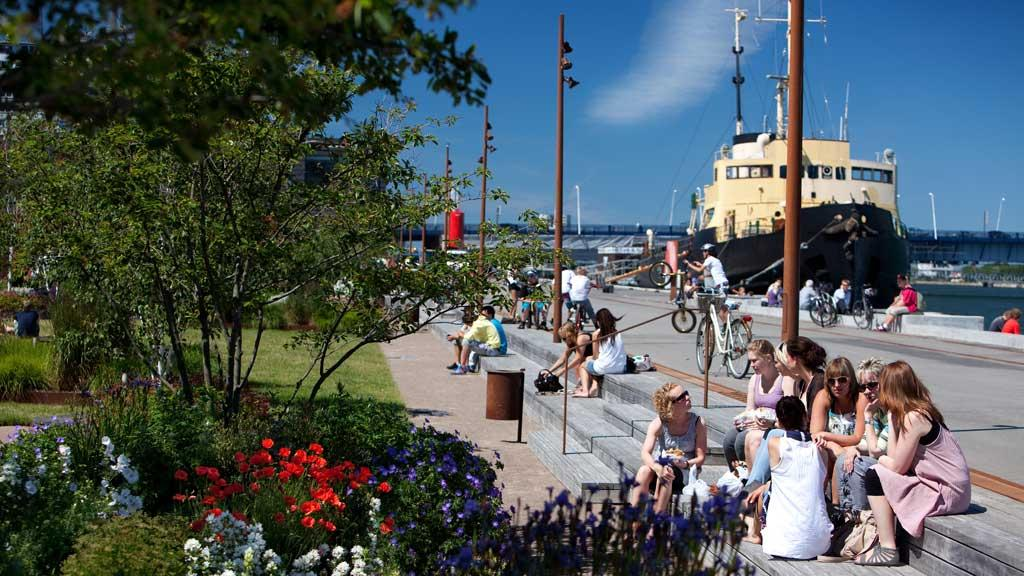
\includegraphics[width=0.90\textwidth]{billeder/aalborghavnefront}
\vspace{4cm}

\vspace{2cm} 
\textsc{\Large P2 Projekt \\
Gruppe A401 \\
Software\\
Aalborg Universitet\\
Den 27. maj 2015\\}
\end{flushright}

\cleardoublepage												% Indsaetter tom side, saa naeste kapitel starter paa hoejre side (hvis noedvendigt)
% Dette er LaTeX-versionen af titelbladet for TNB studenterrapporter
% Filen kræver:
% Universitetets logo:  AAU-logo-stud-UK eller AAU-logo-stud-DK
% Synopsis: En fil ved navn synopsis.tex

% Udarbejdet af: Jesper Nørgaard (jesper@noergaard.eu) 10. april 2012

\phantomsection
\pdfbookmark[0]{Titelblad}{titelblad}
\thispagestyle{empty}

\begin{minipage}[t]{0.48\textwidth}
\vspace*{-25pt}			%\vspace*{-9pt}

\includegraphics[height=4cm]{billeder/AAU-logo-stud-DK-RGB}
\end{minipage}
\hfill
\begin{minipage}[t]{0.48\textwidth}
{\small 
\textbf{Første Studieår v/ Det Teknisk-}\\
\textbf{Naturvidenskabelige Fakultet}  \\
Software \\
Strandvejen 12-14 \\
9000 Aalborg \\}
\end{minipage}

\vspace*{1cm}

\begin{minipage}[t]{0.48\textwidth}
\textbf{Titel:} \\[5pt]\bigskip\hspace{2ex}
Orienteringsløb

\textbf{Projekt:} \\[5pt]\bigskip\hspace{2ex}
P2-projekt

\textbf{Projektperiode:} \\[5pt]\bigskip\hspace{2ex}
Februar 2015 - Maj 2015

\textbf{Projektgruppe:} \\[5pt]\bigskip\hspace{2ex}
A401	

\textbf{Deltagere:} \\[5pt]\hspace*{2ex}
Christian Dannesboe \\\hspace*{2ex}
Frederik Børsting Lund \\\hspace*{2ex}
Karrar Al-Sami \\\hspace*{2ex}
Mark Kloch Haurum \\\hspace*{2ex}
Søren Lyng \\\hspace*{2ex}

\textbf{Hovedvejleder:} \\[5pt]\hspace*{2ex}
Jacob Nørbjerg \\\bigskip\hspace{2ex}

\hspace*{2ex}
\bigskip\hspace{2ex}
\vspace*{1cm}

\textbf{Oplagstal: 10} \\
\textbf{Sidetal: 65} \\
\textbf{Appendiks: 2} \\ 
\textbf{Afsluttet 27-05-2015}

\end{minipage}
\hfill
\begin{minipage}[t]{0.483\textwidth}
Synopsis: \\[5pt]
\fbox{\parbox{7cm}{\bigskipProjektet er udafbejdet ud fra projektoplægget "Bedre rutevejledning i Google Maps". Frem for en rute mellem ét punkt til ét andet punkt, ønkes en flerpunktsrute. Som case har gruppen overvejet forskellige grupper, hvor valget faldt på at fokusere på turister. Formålet med projektet er at lave en interessant flerpunktsrute, dog vil gruppen ikke diktere hvad den interessante rute er, derfor kan brugeren selv tilføje attraktioner, som vil udgøre personens interessante rute. Der er blevet undersøgt forskellige algoritmer, til at finde en relativ kort rute mellem attraktionerne, så ruten både vil være brugerens interessante rute, samt den forholdsvis korteste rute.
\bigskip}}
\end{minipage}

\vfill

{\footnotesize\itshape Rapportens indhold er frit tilgængeligt, men offentliggørelse (med kildeangivelse) må kun ske efter aftale med forfatterne.}

% Rapportens indhold er frit tilgængeligt, men offentliggørelse (med kildeangivelse) må kun ske efter aftale med forfatterne.
% The content of the report is freely available, but publication (with source reference) may only take place in agreement with the authors.

%\cleardoublepage
\phantom{Luft}

\phantom{Luft}
\vspace{5 cm}
\begin{table}[H]
	\vspace{3 cm}
	\centering
		\begin{tabular}{c c c}
			\underline{\phantom{mmmmmmmmmmmmmm}} & \underline{\phantom{mmmmmmmmmmmmmm}} & \underline{\phantom{mmmmmmmmmmmmmm}} \\
			Christian Dannesboe			& Frederik Børsting Lund 		& Karrar Al-Sami 			\\
			&&\\
			&&\\
			\underline{\phantom{mmmmmmmmmmmmmm}} &  \underline{\phantom{mmmmmmmmmmmmmm}} \\
			Mark Kloch Haurum			& Søren Lyng \\										
		\end{tabular}
\end{table}
\newpage
{\Huge\textbf{Forord}}
Dette projekt er udarbejdet i samarbejde mellem fem software-studerende på andet semester fra Det Teknisk-Videnskabelige Fakultet på Aalborg Universitet. 

I udarbejdelsen af projektet, har gruppen taget udgangspunkt i Aalborg-modellen, i form af problem- og projektbaseret læring. Der tages udgangspunkt i et problem, hvor læringen sker i form af projektarbejde i grupper.

Gruppen vil gerne takke vejlederen Jacob Nørbjerg, for hans vejledning gennem hele projekt forløbet. Derudover vil gruppen gerne takke Claus Bobach for deltagelsen i interviewet, der gav indblik i o-løbstræning..... FORSÆTTES!

{\Huge\textbf{Læsevejledning}}

{\Large\textbf{Kildehenvisning}}\newline
I dette projekt bruges Harvard-metoden, også kendt som Chicago-metoden, til kilde henvisning. Hvis der henvises til en bestemt kilde, efter eksempelvis en sætning, påstand eller et citat, henvises der på følgende måde: Sætning/påstand/citat [Forfatter, udgivelsesår].\newline
Hvis kilden anvendes til hele afsnit, sættes kildehenvisningen efter punktummet, således: Afsnit.[Forfatter, udgivelsesår]\newline
I afsnittet ”Litteratur” vil kilde henvisningerne blive sorteret i alfabetisk rækkefølge. Hvis det eksempelvis var en hjemmeside der blev brugt som kilde, ville det se således ud: \newline
\textbf{Kilde henvisningen fra rapporten}. Forfatter. \textit{Titel}. URL. Udgivelsesår. Dato siden er set og evt. sidetal.

\textbf{Dansk Idrætsforbund, 2013}. Dansk Idrætsforbund. \textit{Medlemstal}.\newline http://www.dif.dk/da/om\_dif/medlemstal, 2013. Set d. 27/2-2015.

Hvis nogle af disse informationer mangler, eksempelvis udgivelsesår, udelades de.

{\Large\textbf{Figurhenvisning}} \newline
Igennem rapporten vil der blive henvist til figurer og illustrationer, hvor det vil blive anvist ud fra hvilket afsnit det befinder sig i, samt hvilket nummer figuren er i det omtalte afsnit. Herudover skal der være en beskrivende tekst, der forklarer figuren, eksempelvis:
\begin{flushleft}
	{\LARGE\textbf{Figur 2, afsnit 5: Figurtekst}}\newline
	Figur 5.2: Figurbeskrivelse
\end{flushleft}

\cleardoublepage

%%%% Indholdsfortegnelse (TOC) %%%%

\phantomsection													% Kunstigt afsnit, som hyperlinks kan 'holde fast i'
\pdfbookmark[0]{Indholdsfortegnelse}{indhold}					% Tildeler en klikbar bookmark til den endelige PDF
\tableofcontents*												% Indholdsfortegnelsen (kaldet ToC) 

%\addtocontents{toc}{\protect\newpage}							% Fremtvinger sideskift i ToC hvis noedvendig (der hvor koden placeres)


\mainmatter														% Hovedindhold - nummereres fra side 1

%%%% Rapportindhold %%%% 										% Rapportindholdet boer IKKE indeholde broedtekst - KUN includede filer!

%% Indledende %%												% Opdel evt. i passende afsnit for overblikkets skyld

\chapter{Indledning}
Der findes mange forskellige typer af foreninger i Danmark, hvor nogle er større end andre, og derfor har flere ressourcer til rådighed. Derfor skal mindre foreninger være mere ressource bevidste end andre, og arbejdsbyrden på de enkelte medlemmer kan være stor.\newline
Denne rapport vil forholde sig til orienteringsløb i mindre foreninger, hvor der i Danmark er 76 foreninger med omtrent 7.000 medlemmer \citep{DIF}. Igennem et interview med Jens Børsting, som har løbet og været engageret i o-løb i over 30 år, blev det konkluderet, at der er meget arbejde for medlemmerne i o-løbsforeninger, og at det er begrænset hvor meget software der findes til at hjælpe o-løbere. \newline
I et orienteringsløb skal en løber med kort og kompas hurtigst muligt finde et antal forudbestemte poster, typisk i en skov. Da løberne undervejs er svære at holde under opsyn, er det ikke attraktivt at være tilskuer til et o-løb. Der er samtidigt ikke mange unge o-løbere til trods for, at Danmark har nogle af verdens bedste o-løbere \citep{RANK}. \newline
Hidtil har posterne været opsat fysisk, og ruten der er tiltænkt løbet er planlagt på forhånd. Dette arbejde indebærer flere timers arbejde både før og efter en træningsgang eller løb, da posterne også skal hentes efterfølgende. Derudover kan det være svært at sammenligne de vejvalg, den enkelte løber har taget på ruten, da sammenligning kun kan ske ud fra løbernes hukommelse. Dette gør det svært for træneren at fortælle hvad løberen kunne have gjort anderledes, medmindre træneren løber efter løberen, hvilket vil sige at løberen har spotter på. Løberen kan heller ikke sammenligne sine vejvalg med de andre løbere, for at finde svagheder i sit eget løb.\newline 
For amatør o-løbere er det svært at udvikle sig, grundet den begrænsede feedback løberen kan få fra træningen.\newline
Den initierende problemstilling i dette projekt lyder derfor sådan:\newline
Hvordan kan planlægningen, afviklingen og opfølgningen af træningen for amatør o-løbere forbedres/effektiviseres vha. en IT-løsning?
\begin{itemize}
	\item Hvordan foregår en o-løbstræning?
	\item Hvilke problemer forekommer der under en o-løbstræning?
	\item Hvilke teknologiske redskaber bruges til en o-løbstræning?	
\end{itemize} 


% Analyse % 

\chapter{Problemanalyse}
I dette kapitel vil den initierende problemstilling blive analyseret. Dette gøres i form af interessentanalyse der skal hjælpe til at finde de væsentlige interessenter til projektet. På baggrund af interessentanalysen, bliver der foretaget interviews med udvalgte interessenter. Til sidst i kapitlet vil eksisterende løsninger blive beskrevet og analyseret.
\section{O-løb}
O-løb er en sport, hvor det, som så mange andre sportsgrene, gælder om at være hurtigst. I o-løb er det dog ikke så let, som bare at løbe den markerede vej. Det er nemlig op til løberen selv at finde vej, ved hjælp af et kort, og måske et kompas.  
Inden løbet starter, bliver alle løbere udstyret med et kort, der med en detaljeret visning af stier, bakker og andre udfordringer i terrænet , viser hvor de forskellige poster befinder sig, som løberen skal nå at besøge, inden vedkommende er færdig. Hvis kortet viser en bestemt rækkefølge posterne skal besøges i, så er det påkrævet at gøre det i den rækkefølge. 
Kortlæsning er en af de vigtigste aspekter ved o-løb. Det gør løberen i stand til at finde rundt, optimere sin rute, vælge den bedste vej rundt om forhindring. ”Vi kan med god ret sige, at det er her sjælen i sporten ligger gemt”, som Dansk Orienteringsforbund skriver.   
Ved hver post, står en  orange/hvis skærm. På skærmen er oplyst et nummer, så det er muligt at tjekke om man nu har fundet den rigtige. Desuden er der ved mange løb, i hvert fald mange af dem der ikke blot er træningsløb, opstillet elektronisk poster der husker hvornår du har været ved posterne. 
Der findes en række forskellige discipliner indenfor o-løb. Først er der Sprint, Mellem, Lang og  Ultralang, der er enkeltmandsløb, hvor den eneste forskel er distancen der løbes. Sprint er den korteste, og ofte afvikles i byer for at gøre det så simpelt og hurtigt som muligt, og Ultralang er den længste, hvor vindertiden typisk er højere end ved maratonløb. 
Udover standardløbene, findes også Nat, Stafet og Hold, der adskiller sig ved, som stafet og hold, at have flere løbere, eller ved natløb, ved at foregå om natten. 

\newpage
\section{Begreber}
I dette afsnit vil nogle begreber og fagord inden for orienteringsløb, som bliver brugt i løbet af projektet, blive forklaret.

\textbf{Orienteringsløb}\newline
Orienteringsløb, eller forkortet o-løb, er en sportsgren der går ud på at finde vej i terræn. \newline
De typer orienteringsløb de fleste kender er det som kaldes ”lang” og ”mellem”, der indikere distancerne, hvilket vil være de discipliner der vil blive taget udgangspunkt i, i dette projekt.\newline
En lang er en distance på syv til otte kilometer, som er den normale disciplin. Mellem er derimod kortere, hvor der er flere poster og retningsskift.\newline
Kort sagt gælder orienteringsløb om at finde en række poster i et terræn, som kunne være en skov, vha. et kort og et kompas. Et af de vigtige elementer i orienteringsløb er kortet. Kortet fremstilles af de lokale orienteringsklubber og deres medlemmer, vha. eksisterende kort, luftfotos og laserscannede højdekurver. Løberne skal kunne aflæse kortet, for at finde det hurtigste og sikreste vejvalg mellem punkterne, da det ud fra kortet er muligt, at læse hvordan terrænet ser ud. \citep{DOF}   

\textbf{EMIT brik systemet}\newline
Til tidtagning af o-løb bruges oftest EMIT brikken, som stammer fra Norge. EMIT brikken er en lille firkantet brik, på ca. 5x10x1cm, som løberen har i sin håndflade. Ved hver post er en kontrol enhed, der gemmer postens nummer og tiden i brikken. Ved endt løb aflæses brikken og tiderne kan skrives ud. 

\textbf{Orienteringsløbere}\newline
En orienteringsløber, eller o-løber, er en person der deltager i o-løb, uanset om det er på professionelt niveau, eller som en fritidsaktivitet.

\textbf{Stræk}\newline
Et stræk er stykket mellem to poster i et orienteringsløb. Dette er oftest meget individuelt, da løberne ikke nødvendigvis tager den samme rute for at nå fra en post til en anden.

\textbf{Delstræk}\newline
Mindre dele af et stræk, der ikke er fra post til post. 

\textbf{Stræktider}\newline
Tiden det tog at komme fra en post til en anden.\newline


\subsection{Typisk o-løbs træning}
I dette afsnit vil en typisk o-løbs træning blive beskrevet, og der bliver analyseret på nogle af de problemer o-løbere støder på i forbindelse med en træning. Afsnittet er udarbejdet ud fra information af Jens Børsting.

Før en træningssession kan starte, skal der først søges tilladelse hos Naturstyrelsen, til den skov, hvor der skal løbes. \newline
Til hver træning beslutter træneren hvilke fokuspunkter der skal trænes, eksempelvis tekniske fokuspunkter, som højdekurvelæsning, eller mere fysisk som konditionstræning. Herefter planlægges løbet i et computerprogram, som f.eks. Condes, hvor de enkelte ruter/baner tegnes på orienteringskort. Desuden udarbejdes der også et orienteringskort, som bruges til udsætning af poster til træningen. Det meste af dette arbejde kan gøres hjemmefra, dog er det ofte sekretæren i klubben, der står for at printe orienteringskortene. Hele planlægningen af træningen tager omkring to timer. Dagen før træningen, bliver alle poster typisk hentet i klubhuset og sat ud i skoven, denne proces tager omkring to timer. Der er flere forskellige typer af poster. De mest simple er en skærm, altså bare en farvet stofkasse, der blot indikere hvor posten er. Der findes også en større og besværligere udgave, der er en pind i jorden på ca. 1m, med en skærm omkring og en elektronisk aflæser på toppen, som løberne kan bruge EMIT brikker til(der kan læses mere om EMIT brikker i afsnit 2.3.2). Det tager cirka en times ekstra arbejde hvis der vælges en af de større elektroniske poster.\newline
På dagen mødes alle løbere og får instruktion om løbets fokuspunkter. Herefter uddeles baner alt efter niveau og kondition, hvor der er typisk 3-7 baner at vælge imellem. Løberne bliver derefter sendt ud i skoven, med et kort, kompas og evt. EMIT brik hvis det er en mulighed. Når løberne er færdige med deres tur, får de en udskrift over hvilke poster de har været ved, og hvor lang tid der er gået mellem hver post, hvis EMIT brikkerne har været taget i brug.
Efter løbeturen, har løberne mulighed for at evaluere deres tur, ved at snakke sammen med andre løbere, og sammenligne vejvalg og stræktider. Vejvalg foregår udelukkende efter hukommelse og det er ikke muligt at se forskel i hastighed på delstræk, kun hele stræk mellem 2 poster. 
Efter træning, eller dagen efter, skal alle poster samles ind igen og pakkes ind i klubhuset.\newline

Hvordan en typisk o-løbstræning foregår afhænger af klubben og løberne, men som en generel hovedregel, kan det siges at der inden en træning er blevet lavet 3 eller flere ruter der kan løbe. Hvordan tidstagningen foregår, og om der overhovedet er nogen form for tidstagning til træningen. Derfor 

\subsubsection{Problemer}
Ud fra interviewet med Claus Bobach, er to problemstillinger blevet belyst, i forbindelse med en typisk o-løbs træning. Disse to problemer, er forberedelsestiden og evalueringen af træningen. Problemerne er her beskrevet.

Der bliver brugt en time til halvanden på forberedelse af en træning eller et løb, og derudover skal alle posterne sættes ud, og efterfølgende pakkes sammen igen. Dette svarer til yderligere 2,5 til 3 timers arbejde. \newline
Problemet er at der skal folk til at gøre det, og i små frivillige foreninger, er der ikke nogen der kan blive betalt løn for at gøre det, men der skal udelukkende satses på frivillige, der gider at tage ansvaret for det. \newline
Derudover er det et endnu større arbejde, hvis der ønskes en form for tidtagning på posterne, da de elektroniske poster tager en time mere for henholdsvis at stille op og samle sammen. 

Problemet med evaluering af træningen for både træner og deltagere, er problemerne med at kunne se tider på delstræk, og vejvalg. Bare fordi to personer har løbet cirka lige hurtigt mellem to poster, behøver det ikke at betyde at de begge har fundet den samme gode vej. Det kan fx være at den ene var hurtigere på den første del på grund af vejvalg, mens den anden var hurtig på den sidste del, og det i virkeligheden ville være meget hurtigere at vælge en kombination af de to ruter. Som det gøres nu sammenlignes der stort set kun ud fra de enkelte løberes hukommelse, hvilket gør sammenligningen upræcis. Nogle løbere evaluere selv derhjemme ud fra GPS dataene fra deres GPS ure. Konsekvensen ved dette er at der ikke sammenlignes med andre løbere, og dermed vil vedkommende have svært ved at se hvor der kunne være taget bedre vejvalg på ruten.

I samarbejde med træner Claus Bobach, har gruppen belyst to problemstillinger, der opstår i forbindelse med en typisk o-løbs træning. Disse to problemer, er først det tidskrævende arbejde, der ligger i forberedelsen af en træning, og dernæst den mangel på evaluering, der foretages, hvis ikke løberne selv ligger en aktiv indsats i at huske deres vejvalg, og få snakket med de andre løbere. 
\section{Interessentanalyse}
I dette afsnit indflydelses- og medvirken matrixen blive anvendt, for at undersøge og prioritere interessenter for dette projekt. Dette undersøges for, at finde ressourcepersoner som gruppen kan gøre brug af gennem interviews. Disse personer vil være respondentgruppen til undersøgelse af den initierende problemstilling.
Jens Børsting nævnte i interviewet, at o-løbere er interessenter, da de ønsker en IT-løsning til sammenligning af løb, samt o-løbs trænere er interessenter, da de ønsker bedre træning, samt nedsat arbejdsbyrde.

Gruppen vil i dette afsnit undersøge diverse personer/grupper, der kan fungere som interessenter i projektet, altså en person der vil have nytte af eller kan bidrage til projektet.

\subsection{Aktører}
I dette projekt har gruppen fundet tre aktører med hjælp fra Jens Børsting, som gruppen mener er relevante til projektet. De forskellige aktører er henholdsvis o-løberne, trænerne og sportens forbund og foreninger. 

\subsubsection{O-løbere}
For at den enkelte o-løber skal kunne forbedre sig, er det vigtig at kunne sammenligne løberens rute detaljeret med andre. Lige nu er tiderne mellem hver post (stræktiderne) det eneste der kan sammenlignes og analyseres på. Her er det interessant for løberen at kigge på vejvalg og hastighed mellem posterne, og endda helt ned til de forskellige faser af delstrækkene. Til dette mangler der mere detaljeret data om løbet. Problemet håndteres i dag ved at sammenligne skemaer med stræktider og hvis muligt manuelt indtegne vejvalg på kortet efter løberens hukommelse. Derfor har den enkelte o-løber interesse i dette projekt, da der arbejdes med afvikling og opfølgning af træningen. 

\subsubsection{Træneren}
Træneren har interesse i at gøre de enkelte løbere bedre, træneren har derfor også interesse i at mindske arbejdet på planlægning og forberedelse af træningen, da der bruges meget tid med dette. Samtidigt vil træneren gerne kunne analysere den enkelte løbers tur detaljeret, ved at sammenligne løberens rute med andre løberes rute. Hvis løberen ikke kan huske hvor vedkommende har løbet, eller var faret vild, har træneren svært ved at give sikker og brugbar kritik, da det ikke kan ses på tiderne, præcis hvor den enkelte løber har været. Trænere har derfor interesse i et værktøj som kan hjælpe med planlægning og afviklingen af træningen, samt evaluering af den enkelte løbers tur.

\subsubsection{Forbund og foreninger}
O-løbernes forbund hedder Dansk Orienterings Forbund, også kaldt for DOF, som ligger under Dansk Idrætsforbund, DIF. Der er i alt 76 foreninger i DOF, med lidt under 7.000 medlemmer\citep{DIF}. DOF er med til at drive landsholdet, samt står for talentudviklingen inden for orienteringsløb. Dette gør DOF og foreningerne til interessenter i dette projekt, da de bl.a. ønsker deres løbere skal blive så gode som mulige. Derudover kunne de have nogle krav til en evt. løsning. \citep{DIF}

\subsubsection{Frivillige}
I interviewet med Claus Bobach nævnte han, at det var frivillige der satte posterne ud for ham. Derudover er mange af de frivillige engageret i o-løb, da de er villige til at lave et strykke ubetalt arbejde, for at holde gang i klubben. Eksempelvis i Claus' klub, har de nogle der sørger for mad og drikke efter træninger, samt før nævnt hjælper til med posterne.


\subsection{Prioriteringen}
Ved prioritering af interessenter, bliver indflydelse- og medvirken matrixen anvendt. Denne matrice deles op i fire rum, hvor hvert rum er scaleret efter ”indflydelse på projektet” og ”afgørende medvirken i projektet”. Dette giver rum for diskussion af de enkelte interessenter, for at undersøge hvilke interessenter, der skal tages kontakt til, for at få svar på den initierende problemstilling.
Gruppen har i denne rapport meget få interessenter, hvilket medfører, at de enkelte interessenter hurtigt bliver ressourcepersoner.

\textbf{Eksterne interessenter} har hverken en stor indflydelse eller en stor medvirken i projektet. Det betyder at der ikke nødvendigvis skal tages stor hensyn til denne gruppe af interessenter.\newline 
\textbf{Den grå eminence} har stor mulighed for at påvirke beslutninger i projektet, men deres medvirken er ikke særlig stor i projektet, dette vil ofte være en person med en magtfuld stilling eller ledelses position. \newline
\textbf{Gidsler} har ikke stor mulighed for at træffe beslutninger i projektet, men deres aktive medvirken er vigtig for projektet.\newline
\textbf{Resourcepersoner} har både stor indflydelse og stor medvirken, da det er denne gruppe der skal inddrages i projektet. Denne gruppe har både erfaring eller faglige kompetencer indenfor området. \newline
  
O-løbere er i dette projektet sat som ressourceperson, da de kan give råd og vejledning til, hvordan deres træning og løb fungere, samt undersøge om der er ting der kan forbedre o-løbernes løb. Dette gælder både inden løb og efter løbet.

Trænere er sat som ressourceperson for projektet, da de ligesom o-løberne har et stort indblik i hvordan orienteringsløb fungere, og hvordan det måske kan optimeres eller forbedres. 

DOF og foreningerne er i dette projekt grå eminence, da de kan have en indflydelse på projektet. Herudover kan de have nogle krav og regler til en løsning. Deres medvirken er dog ikke nødvendig for at projektet skal kunne blive en succes.

I dette projekt har gruppen valgt at placere de frivillige som gidsler. Da de frivillige ikke har nogen indflydelse på hvordan projektet bliver lavet, men de laveer stadig et stykke arbejde som er værd at tænke over i løsningen.    

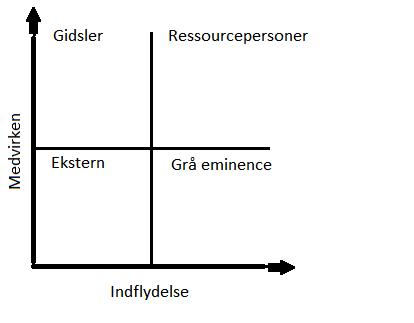
\includegraphics[width=0.70\textwidth]{billeder/matrix}
\vspace{0.20cm}

\subsubsection{Opsummering}
Ud fra interessentanalysen, er gruppen kommet frem til at o-løberne og trænerne, er de vigtigste interessenter, og er derfor også blevet sat som ressourcepersoner i dette projekt. Derfor har gruppen valgt at kontakte de to grupper af interessenter, og gennemføre et interview med dem. 

%\section{Spørgeskema}


\subsection{Udformning}


\subsection{Opsummering}

%\section{Interviewet}


\subsection{Udformning}


\subsection{Resultatbehandling}


\subsection{Opsummering}


\chapter{Eksisterende løsninger}
I dette afsnit vil de nuværende IT-løsninger blive forklaret, som har indvirken på problematikker vedrørende o-løbstræning. 

\section{Endomondo}
”Den succesrige danske løbeapplikation, Endomondo, er blevet solgt til et stort, amerikansk selskab”, sådan lyder nyhederne om denne applikation til Smart-phones, som bruges af omkring 25 millioner mennesker. \citep{ENDO}

Endomondo er en applikation som bruges til løb, hvori en træningsplan kan udformes. App’en vil her have to versioner, en gratis og en udvidelses-version som kan købes. Endomondo bruger Google Maps som kort i deres app\citep{ENDOMAPS}.Funktionaliteten der her vil blive beskrevet er for gratis versionen: Hovedmenu med otte funktioner:
\begin{itemize}
\item Newsfeed, som bruges til at kommunikere med andre brugere af Endomondo, hvor brugere kan opmuntre, samt udfordre hinanden til
\item Notifikationer, hvor brugeren kan se sine udfordringer og lignende fra andre brugere, her kan brugeren acceptere eller afslå udfordringer.
\item Historik, hvor tidligere løb oplagres til genvisning og statistik.
\item Kort, hvor brugeren ved hjælp af mobilens GPS-enhed kan få et kort over ruten der er løbet. Kortet er standardiseret, og viser personens placering og rute.
\item ”Opgrader-nu”, hvor gratis versionen kan betales til opgradering.
\item Venner er en funktion, hvor brugeren kan overvære venner fra sociale medier.
\item Træningsplanen bruges til at indstille app’ens hjælpefunktioner til træning, hvor brugeren selv sætter mål for træningen, intensiteten ved træningen, og hvilken typen af træning der udøves.
\item Indstillinger er en funktion der findes i alle programmer, hvor de generelle indstillinger for programmet kan tilpasses brugeren.
\end{itemize}
Dette er en velfungerende app til formålet, løb og træningsplan, men i det en O-løber skal bruge visningen af løbet på et kort som brugeren selv har fra det specifikke O-løb, kan dette blive problematisk, da brugeren ikke selv kan sætte kort ind i programmet. 


\section{EMIT-brikker}
En EMIT-brik, er et elektronisk apparat, der kan registrere hvilke poster der besøges. EMIT-brikken sidder fast på fingeren, ved hjælp af et elastik. \newline
Måden en EMIT-brik fungere på, er at den stilles på en startpost ca. 5 sekunder før løbet bliver sat i gang. Dette vil genstarte EMIT-brikken, således at den kan notere de rigtige tider. 
Ved hver post, der skal besøges, er der en kontrolpost, der ligner startposten, som EMIT-brikken skal lægges på i ca. ½ sekund. Dette vil registrere hvor lang tid der er gået mellem forrige post og nuværende post. \newline
Til sidst i løbet, vil der være en målpost, hvor EMIT-brikken endnu engang skal lægges på, således at den sidste tid bliver noteret. 
Herefter skal EMIT-brikken afleveres til de ansvarlige, som derefter vil give løberen en udskrift af tiderne. Disse tider kan så derefter anvendes til sammenligning og diskussion med andre løbere.\citep{OOK}

\section{QuickRoute}
Igennem gruppens interview, beskrev Claus, at QuickRoute er en eksisterende løsning på kortlæggelse og rute visning. Denne løsning kommer på bekostning af et Garmin ur, eller andre GPS enheder, som kan generere en GPX fil over ruten. I QuickRoute kan et kort fra Ocad lægges ind, og ved hjælp af Garmin ure kan en route blive vist, hvor forskellige parametre kan blive afbildet. Hastighed, minutter per kilometer, hjertefrekvens, højdemeter og afvigelse fra retningen mellem to punkter kan blive afbildet. Dette bliver vist ved en farve-kode der følger ruten, og gennem hele ruten vil denne farvekode variere efter hvert interval af GPS-signal. Med den rigtige serie af Garmin ure, kan der tilmed tages tid på, hvornår en post er nået, så en statistisk model kan beskrive tiderne mellem posterne. Hvis musen holdes over et punkt på ruten, kan følgende information om punktet vises: Klokkeslæt, tid brugt i alt på rute, samlet distance løbet til det punkt, nuværende minutter per kilometer, nuværende hastighed i km/t, nuværende hjertefrekvens, nuværende højdemeter, nuværende afvigelse mellem to punkter, nuværende længde- og breddegrader. Mange af disse informationer kan afbildes statistisk både grafisk og på et histogram \citep{QR}.\newline
Til at toppe alt dette af, kan det efterfølgende integreres på Google Earth, så der kan ses en 3D model af ruten der er brugt. 
Denne løsning er meget gennemført, hvor mange funktioner kan benyttes, dog kan antallet af funktioner og parametre virke overflødig for en amatør o-løber, og der kan være for mange informationer. For en rutineret eller professionel o-løber vil denne løsning give et godt indblik i, hvordan løbet er foregået og hvor personen kan udvikle sig.


\section{TracTrac}
TracTrac er en samlet løsning til livetracking med replayfunktion af forskellige sport events. Til dette bruges TracTrac's egne GPS enheder. Disse er ca. på størrelse med en cigaretpakke og vejer 113 gram.\newline
TracTrac bruges til o-løb så der live kan følges med i hvor o-løberne er ude i terrænet, som f. eks. Til stævner og konkurrencer. Derudover bruges TracTrac i høj grad til at analysere de enkelte løberes ture efter de har løbet, da TracTrac har en velfungerende replay funktion. 

Når TracTrac skal bruges i forbindelse med o-løb, laves der først et o-løbskort som oploades til TracTracs servere. Derefter indsættes præcise punkter på kortet som repræsentere hvor hver enkelt post ligger, så TracTrac kender positionerne på alle posterne. Herefter skal hver enkelt GPS enheds nummer sættes sammen med en løber, så det bliver tydeligt hvem der løber hvor. Under løbet sender GPS enhederne deres position til serverne som viser disse på kortet. Alt dette sker live. En af funktionerne som gør TracTrac ekstra brugbar i forbindelse med o-løb, er dens mulighed for at flytte løbere tilbage til start og afspille deres tur samtidig, så man kan se præcist hvordan de løb i forhold til hinanden, selvom de i virkeligheden startede forskudt. Dette kan også gøres selvom løbet er live. En løber der er foran kan flyttes tilbage så vedkommende løber samme stræk som en anden løber som er startet senere. Dette giver mulighed for grundig analyse og sammenligning af løbernes vejvalg og hastighed, både under og efter løbet.\newline
TracTrac kan stort set alt der er brug for til live visning og analyse af o-løb. Selve GPS-enheden koster 150EU, altså lige godt 1116DKK. Derudover skal der bruges et sim, data kost og enhedslicens til 88EU om året pr. enhed, hvilket vil svare til ca. 650DKK. Som det sidste skal en system-licens bruges, denne koster 990EU årligt, hvilket er 7368DKK. Dette produkt er i sådan en prisklasse, at de små amatør klubber ikke har råd til det. \citep{TTC}


\section{Opsummering}
Ud fra overstående analyse af eksisterende løsninger, mener gruppen der mangler en løsning, der er bygget på mobiltelefonens GPS. Langt de fleste mennesker har en mobil med GPS idag, hvilket vil gøre løsningen billigere, da brugeren ikke skal bruge penge på ekstra udstyr. Endomondo bruger dog mobilens GPS signal, men da der ikke en nogen replay funktion eller mulighed for at indlægge andet end Google Maps' kort bag ruten, er denne løsning ikke velegent til o-løb. 


% Problem %
\chapter{Problembeskrivelse}
I dette kapitel vil problematikkerne i denne problemanalyse blive beskrevet, og herefter vil rapporten afgrænses til et delområde, hvoraf en problemformulering vil uddrages.

\section{Problemafgrænsning}
I udarbejdelsen af problemanalysen blev der fundet to problematikker ved o-løbstræninger. Den første omhandler opsætningen af poster, normale og elektroniske, da trænerne bruger flere timer på at forberede en træning. Posterne skal både ud før træning og samles ind igen efter, hvor de elektroniske poster er mere tidskrævende end de små poster, kun bestående af en lille skærm. Udover dette, er arbejdskraften typisk frivillig, så trænere og andre klubmedlemmer må satse på, at en person frivilligt vælger at bruge tid på forberedelsen. En anden problemstilling er evaluering af løbere under træning. Problematikken opstår i det, at evalueringen kun kan ske ved, at to løbere sætter sig ned og kigger på kortet over den udførte rute, og prøver at erindre hvilke vejvalg de har taget. De har ikke nødvendigvis taget den samme rute, trods de har en næsten ens samlet tid på løbet, hvor den hurtigste rute er muligvis en kombination af de to ruter. Gruppen har valgt at afgrænse sig til evaluering af træningen for o-løbere, da gruppen ser størst potentiale i dette. Dog ser gruppen også en mulighed for at integrere en løsning til opsætning af poster, ved brugen af mobilens GPS. 

Der findes flere eksisterende løsninger, hvor mange anvender GPS-ure, men som beskrevet, er ret dyre. Problematikken er, at der ikke kan sammenlignes vejvalg og tider på et o-løbskort, da dette skal gøres efterfølgende på computeren. Da Endomondo anvender Google Maps, vil o-løberen blot være i en grøn skov på et kort, så løberen kan ikke se andet end en rute på en grøn plet. EMIT brikker anvendes til tidtagning under træningen, men denne løsning er ikke særligt anvendelig, da den blot giver stræktider, så løbere kan kun evaluere hvor hurtig de er mellem to stræk, men ikke vejvalg. QuickRoute er et godt værktøj til evaluering af løberen, men da denne løsning kræver et GPS-ur, bliver det hurtigt dyrt for en amatør o-løber.
TracTrac er en allerede kendt løsning, men som beskrevet i afsnittet omhandlende løsningen, skal brugere have licens, samt firmaets egne GPS-enheder, hvilket igen bliver for dyrt for de mindre foreninger.

Ud fra problemanalysens resultater, har gruppen konkluderet, at en software løsning skal bruge mobilens GPS, og derved være en billigere løsning end eksempelvis TracTrac. Løsningen skal også kunne indsætte o-løbs kort, så løberne kan se præcist hvor de har været i terrænet, i stedet for at bruge Google Maps som Endomondo. 

Dette kan optimeres betydeligt med en telefonbaseret softwareløsning, hvor der i afsnittet om eksisterende løsninger er blevet beskrevet, at denne løsning skal kunne hjælpe til evaluering af træningen, uden brug af et GPS-ur.

\section{Problemformulering}
Ud fra ovenstående afgrænsning er følgende problemformulering blevet udarbejdet:

Hvordan kan en telefonbaseret softwareløsning optimere evaluering og træning af o-løbere?
\begin{itemize}
	\item Hvordan kan løberne sammenlignes?
	\item Hvordan følges løberen rundt på ruten?
		\item Hvordan kan løsningen gøres brugervenlig?
\end{itemize}


% Problemlosning %
\chapter{Kravspecifikationer}

\section{Optimale løsningsforslag}
Den ideelle løsning vil bestå af to dele, en mobiltelefon med GPS og en website/server som kan vise dataene sendt fra mobilen

Mobilen skal kunne:
\begin{itemize}
	\item Måle, sende og optage GPS positionen på løberen undervejs på ruten.
	\item Tilslutte sig en bestemt bane, som træneren har opsat og lagt på serveren inden træning.
	\item Mobilen må ikke hjælpe løberen undervejs i løbet, med at vise positionen på ruten.
\end{itemize}

Websitet/serveren skal kunne:
\begin{itemize}
	\item Opsætte baner inden løbet.
	\item Vise løbernes position på kortet.
	\item Vise diverse statistik og data for løberens tur på banen. Dette vil være tider, afstande og hastigheder, samt en grafisk visning af den rute løberen har løbet.
	\item Sammenligne to løberes tur på samme rute, eller sammenligne med banens gennemsnit i forhold til statistik/rådata.
	\item Vise et grafisk replay af den rute løberen har løbet, med mulighed for at afspille flere løbere samtidig og dermed sammenligne vejvalg.
	\item Være kompatibelt med GPS-ure.
\end{itemize} 

Mobil-appen vil have en simpel brugergrænseflade hvor brugeren vil have mulighed for at vælge den bane vedkommende skal løbe. Herefter vil brugeren have mulighed for at trykke start, hvorefter mobilen kun vil vise hvor lang tid der er brugt indtil videre og en afslut knap. Under løbet sender mobilen løbende data om GPS position og tiden siden start. Når turen er løbet færdig trykker brugere på afslut og appen vil sende de sidste data og vise nogle resultater. Dette kan eksempelvis være tid i alt, højeste hastighed, gennemsnitshastighed, men også data om løberen sammenlignet med andre på samme bane. Dette kan f. eks. være hvor mange sekunder efter den hurtigste vedkommende har brugt på de enkelte stræk.

Inden løbet skal træneren eller arrangøren, kunne uploade den bane som personen har lavet, til serveren. Banerne kan vælges fra appen på mobilen, af de forskellige løbere. Efter løbet skal brugerne som sagt kunne uploade sine resultater til websitet/serveren fra mobil appen, under og efter et endt løb. Disse resultater skal så kunne sammenlignes med de andre løbere, der har løbet den samme bane. Ud over at sammenligne statistik over løberens rute, som beskrevet ovenfor, skal den også kunne vise grafisk den rute som løberen har løbet. Derudover skal der være en replay funktion, så de vejvalg som løberen tager, kan ses. Så kan der indsættes flere løbere på den grafiske visning, så flere løberes vejvalg kan sammenlignes.

\section{Gruppens løsningsforslag}
\subsection {Løsningsstrategi}
Løsningsstrategi til statusseminariet.
\begin{itemize}
\item Først vil gruppen undersøge om det er muligt, med gruppens kompetencer i C\#, at kunne dynamisk importere, vise og bruge o-løbskort til løsningen.
\begin{itemize}
\item Hvis overstående ikke er muligt, vil gruppen forsøge at simulere importen af o-løbskortet, og derved kun arbejde ud fra et kort.
\end{itemize}
\item Hvis et af overstående lykkes, vil gruppen efterfølgende lave forskellige former for grafisk analyse, i form af en replay funktion på kortet. Først med kun en løber, og derefter to til flere løbere, for at kunne sammenligne løberne med hinanden.
\item Hvis de overstående fejler, vil gruppen fokusere på detaljerede tekstbaseret analyse, i form af tider, afstande, hastighed osv. som alle skal kunne sammenlignes mellem andre løbere.
\item Hvis alt andet virker for svært eller uinteressant, har gruppen tænkt på at udarbejde en analyse af nøjagtigheden i mobiltelefonens GPS.
\end{itemize}
Gruppen har valgt at simulere mobil GPS dataene, frem for at bruge tid på at lave en mobilapplikation. I tilfælde af at gruppen skal lave analyse af nøjagtigheden i mobiltelefonens GPS, vil mobil GPS dataene ikke blive simuleret. 
 
Hvis der er tid til overs, vil gruppen bruge muligheden til at implementere virtuelle poster eller delvist virtuelle poster. Med virtuelle poster menes at, at vi med GPS enheden konkludere om løberen har besøgt en bestemt post, og på en eller anden måde giver signal til løberen om dette. Med delvist virtuelle poster menes at, der vil blive sat en fysisk skærm ud på banen for at markere posten som sædvanligt, resten vil fungere som den virtuelle post.





\section{Løsningsstrategi}
I dette afsnit vil planen for programmet blive beskrevet, med en overordnet beskrivelse af løsningsstrategi, samt en beskrivelse af valg mht. værktøjer brugt i udviklingen af programmet.

I henhold til gruppens kravspecifikation, vil GPS dataen til programmet blive simuleret af en app til en smartphone. Gruppen har brugt en app kaldet, myTracks til dette formål. myTracks optager og sender GPS signaler i form af en GPX-fil, som bliver tilsendt via e-mail til brugeren.
Som beskrevet i kravspecifikationen, skal brugeren sørge for at kortet anvendt skal være geostationært. Dette betyder, at der sammen med kortet medfølger en tekstfil med tal, der beskriver kortets placering på jordkloden. Med denne fil kan koordinater beskrevet med UTM-systemet (beskrives i teoriafsnittet), oversættes til pixels, og derved gøre det muligt at tegne afstandstro GPS-ruter på kortet. I dette projekt anvendte gruppen QLandkarteGT til at geostationære et kort, som blev anvendt til udvikling af programmet.

myTracks anvender koordinater i Lat/Long-formatet, hvor det geostationære kort oversætter UTM-koordinater til pixels. Dette betyder, at en konvertering fra Lat/Long til UTM er nødvendig, denne konvertering vil blive beskrevet i teoriafsnittet. 

Programmet vil her bestå af to dele, hvor den første del vil behandle data i form af pixels til at tegne ruter på kortet. Anden del af programmet vil bruge UTM-koordinater til at udregne data over løberne, som f.eks. hastighed og distance.

Til udviklingen af dette program har gruppen valgt at benytte Visual Studios Windows Forms, da gruppen ønsker at have en grafisk brugergrænseflade.
\input{problem/design}
\chapter{Teori} 
I dette kapitel vil de anvendte teorier blive beskrevet. Herunder længde- og breddegrader, Universal Transverse Mercator systemet og konverteringen mellem dem. 

\section{Længde- og breddegrader}
I et geografisk koordinatsystem, er jorden inddelt i længde- og breddekredse. Idet jorden er rund, er disse længde- og breddekredse målt i grader, og de bliver i stedet kaldt længde- og breddegrader. \newline
Længdegrader beskriver de vertikale linjer på verdenskortet på figur 5.1, som går fra nordpolen til sydpolen. Disse bliver også betegnet som meridianer. Meridianen der går gennem Greenwich kaldes nulmeridianen, hvorefter den første vestlige længdegrad bliver udtrykt som 1\textdegree vestlig længde, og det samme gælder for den første østlige længdegrad, som vil være 1\textdegree østlig længde. Disse længdegrader bliver herefter talt op, i hver deres retning. Idet en cirkel er 360\textdegree, er de sidste meridianer på hver sin side af verdenskortet kaldet 180\textdegree østlig/vestlig længde. Det skal desuden også nævnes, at længdekredsene ikke nødvendigvis har den samme afstand, da længdekredsene har mindre indbyrdes afstand jo tættere på polerne de er. \newline
Breddegrader beskriver de horisontale linjer i verdenskortet på figur 5.1. Disse linjer er parallelle med ækvator, og deres indbyrdes afstand bliver derfor hverken mindre eller større, men deres omkreds bliver kortere alt efter hvor tæt på polerne de befinder sig. \citep{LongLat}

\begin{figure} [h]
	\centering
	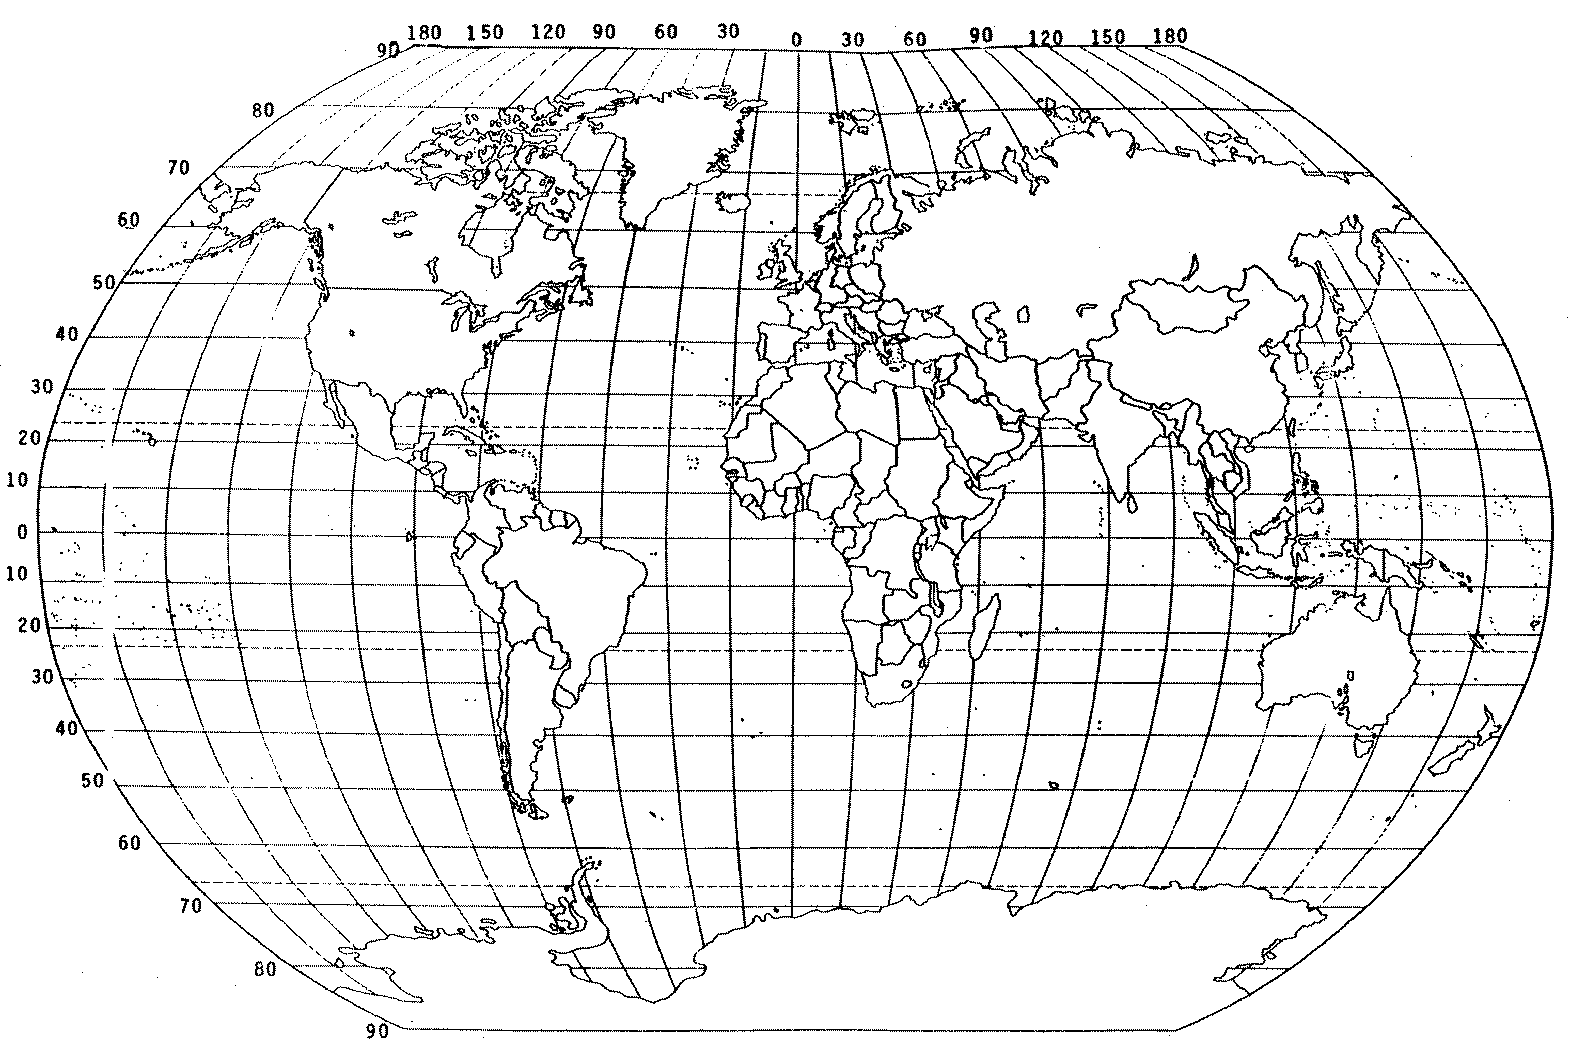
\includegraphics[width=.5\textwidth]{billeder/longlatmap}
	\caption{Verdenskort med længde- og breddegrader}
\end{figure}

\section{Universal Transverse Mercator systemet}
Universal Transverse Mercator systemet, forkortet UTM, er en anden måde at finde lokationer på jordkloden. Denne metode gør brug af, at jordkloden, som reelt set er rund, bliver omformet til en flade, ligesom et stykke papir. Her bliver jorden inddelt i 60 zoner, hvor hver zone er opdelt fra øst til vest, med numre, og syd til nord med bogstaver. De østlige og vestlige, startende fra 180 meridianen, regnes fra vest til øst med 6\textdegree mellemrum. Enkelte zoner er dog blevet gjort bredere eller smallere. Hver zone er nummereret efter deres placering fra vest.\newline
Nordligt og sydligt er inddelt mellem 80\textdegree S bredde, og 84\textdegree N bredde, med en afstand på 8\textdegree, udover en enkelt zone der er 12\textdegree. Hver zone er  navngivet ved et bogstav, fra C-X, startende med C i den sydligste zone.
Alle zonerne i UTM systemet er baseret på en Transverse Mercator projektion, som gør det muligt at kortlægge en region uden stor forvrængning af jordklodens ellers runde form. Hvis jorden blev kortlagt i én stor region, vil dette forårsage store afstands fejlberegninger, da der ikke vil blive taget højde for jordklodens runde form. Det er her at Transverse Mercator projektionen er smart, da den sørger for en lav grad af forvrængning, da det er smalle breddegrader (6\textdegree) der typisk anvendes til zonerne. \newline
Ved positionering gennem UTM systemet, oplyses følgende: Først en zone fra UTM, som f. eks. 17T. Dernæst en østlig og en nordlig afstand. Den østlige udregnes ud fra den centrale meridian. Den centrale meridian er den længdegrad som går igennem midten af zonen. Denne er sat som 500.000 m østlig for at undgå negative tal, dvs. et punkt vest for meridianen giver et tal under 500.000 m, hvor et tal øst for vil være over 500.000 m.  Den nordlige afstand beregnes på følgende måde: Hvis punktet er på den nordlige halvkugle, beregnes den nordlige afstand som afstanden til ækvator. Hvis punktet er på den sydlige halvkugle, beregnes den nordlige afstand som 10,000,000 m minus afstanden til ækvator, for at undgå negative tal. \citep{UTMTeori}

\section{Konvertering}
Som beskrevet i afsnittet løsningsstrategi, er en konvertering mellem længde- og breddegrads systemet til UTM systemet nødvendig. Dog er udregningen ret kompleks og gruppen har derfor valgt ikke at redegøre for formlen i dette teoriafsnit.

Udover konverteringen fra længde- og breddegrads systemet til UTM, skal en konvertering fra UTM til pixels også bruges i projektet. Dette sker ved brugen af en world file. World filen bruges til at oversætte UTM koordinater til pixels på kortet, så det GPS data der loades ind, kan findes på kortet. Dette projekts world file ser således ud:
\begin{description}
	\item[mpx] 0.84964441
	\item[roty] 0.00000000
	\item[rotx] 0.00000000
	\item[mpy] -0.84964441
	\item[x0] 539276.35483168
	\item[y0] 6250863.73506770
\end{description}
\textbf{mpx} - Antal meter pr pixel i x-retning\newline
\textbf{roty} - Rotationsværdi om y-aksen\newline
\textbf{rotx} - Rotationsværdi om x-aksen\newline
\textbf{mpy} - Antal meter pr pixel i y-retning (oftest negativ)\newline
\textbf{x0} - X koordinatet for midten af pixlet i øvereste venstre højrne\newline
\textbf{y0} - Y koordinatet for midten af pixlet i øvereste venstre højrne\newline
Da o-løbskort aldrig er roteret, vil roty og rotx altid være 0, og der vil kigges bort fra disse værdier.

Grunden til at mpy oftest er negativ, er fordi pixels begynder fra øverste venstre hjørne, hvor et UTM koordinatsystemet begynder fra nederste venstre hjørne.Tages der udgangspunkt i figur X kan det forklares således:

\begin{figure} [h]
	\centering
	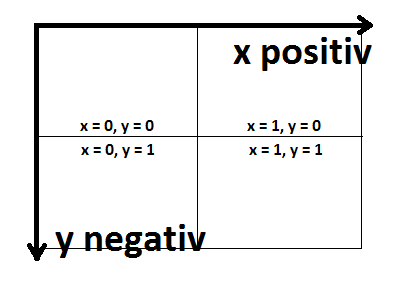
\includegraphics[width=.5\textwidth]{billeder/UTMtilPIXEL}
	\caption{Figur til forklaring af UTM til pixel}
\end{figure}

Koordinatsættet (0,0) vil svare til (x0,y0).
Koordinatsættet (1,0) vil svare til (mpx + x0,y0)
Koordinatsættet (0,1) vil svare til (x0,mpy + y0)
Koordinatsættet (1,1) vil svare til (mpx + x0, mpy + y0)

For at finde pixel-position (x’, y’) ud fra UTM koordinat (x,y) bruges følgende formel:\newline
x’ = (x - x0) / mpx\newline
y’ = (y - y0) / mpy\newline

\subsection{Opsummering}
Længde- og breddegrader og Universal Transverse Mercator systemet er blevet kort forklaret. Gruppen har valgt ikke at forklare den brugte formel i konverteringen fra længde- og breddegrader til UTM koordinater. Det lykkedes at opstille formlen for konverteringen fra UTM koordinater til pixels. Denne teori vil blive brugt i kapitlet “Implementeringen”. 
\chapter{Implementering}
Dette kapitel omhandler det fremstillede programs brugergrænseflade, et afsnit om programstruktur med tilhørende klassebeskrivelse, samt implementeringen af kildekoden.

\section{Brugergrænseflade}
Ved programmets opstart vises det statiske kort som gruppen har valgt at benytte under udviklingen af dette program, samt en load knap. Dette er at finde i tabben “Map View”. Tabben “Data View” vil ikke indeholde noget information ved opstart af programmet. Efter tryk på load knappen,	 popper en dialogbox op, hvorefter brugeren skal vælge den mappe som indeholder løbernes GPX-filer, samt koordinater for posterne til den bane løberne skal løbe. Dette kan ses på figur 6.1.

\begin{figure} [h]
	\centering
	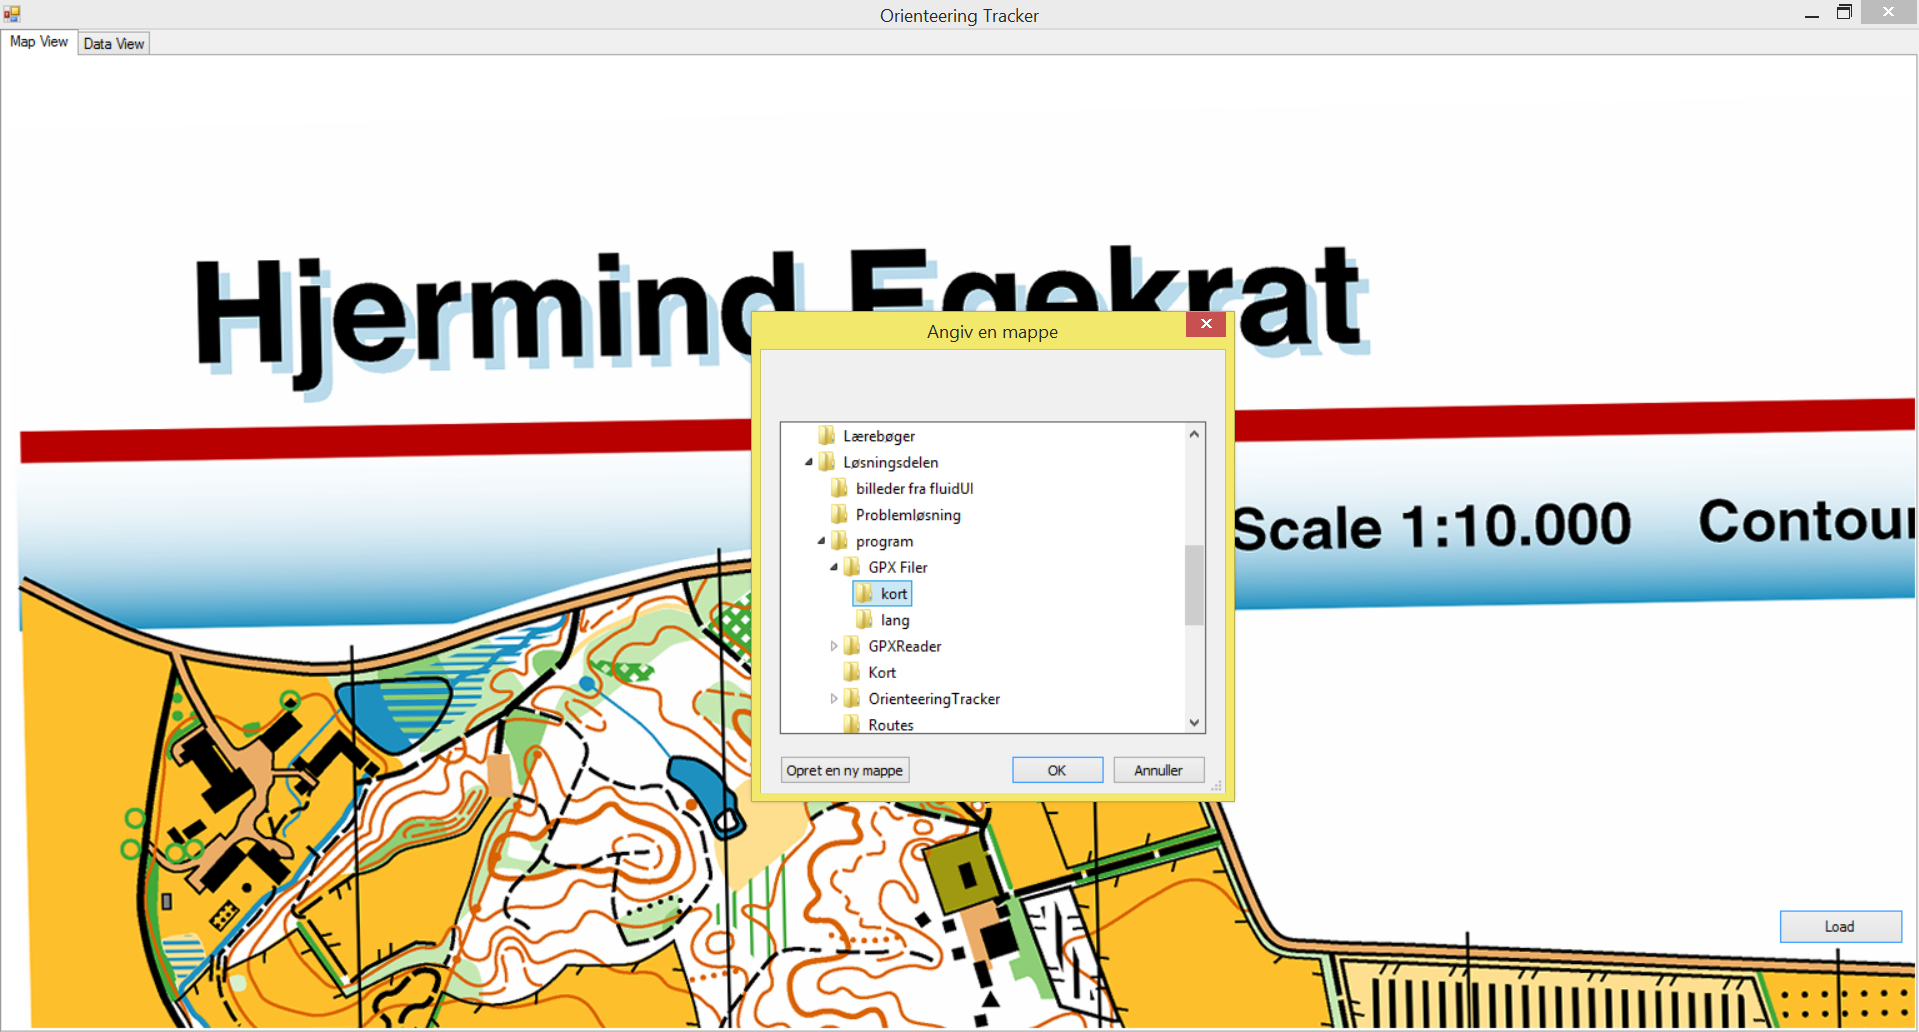
\includegraphics[width=1\textwidth]{billeder/MapView1}
	\caption{Klassediagram over projektets program}
\end{figure}

Når GPX-filer og koordinaterne for posterne er loadet ind i programmet, vil de forskellige mediaplayer funktioner komme frem, som ses på figur 6.2.

\begin{figure} [h]
	\centering
	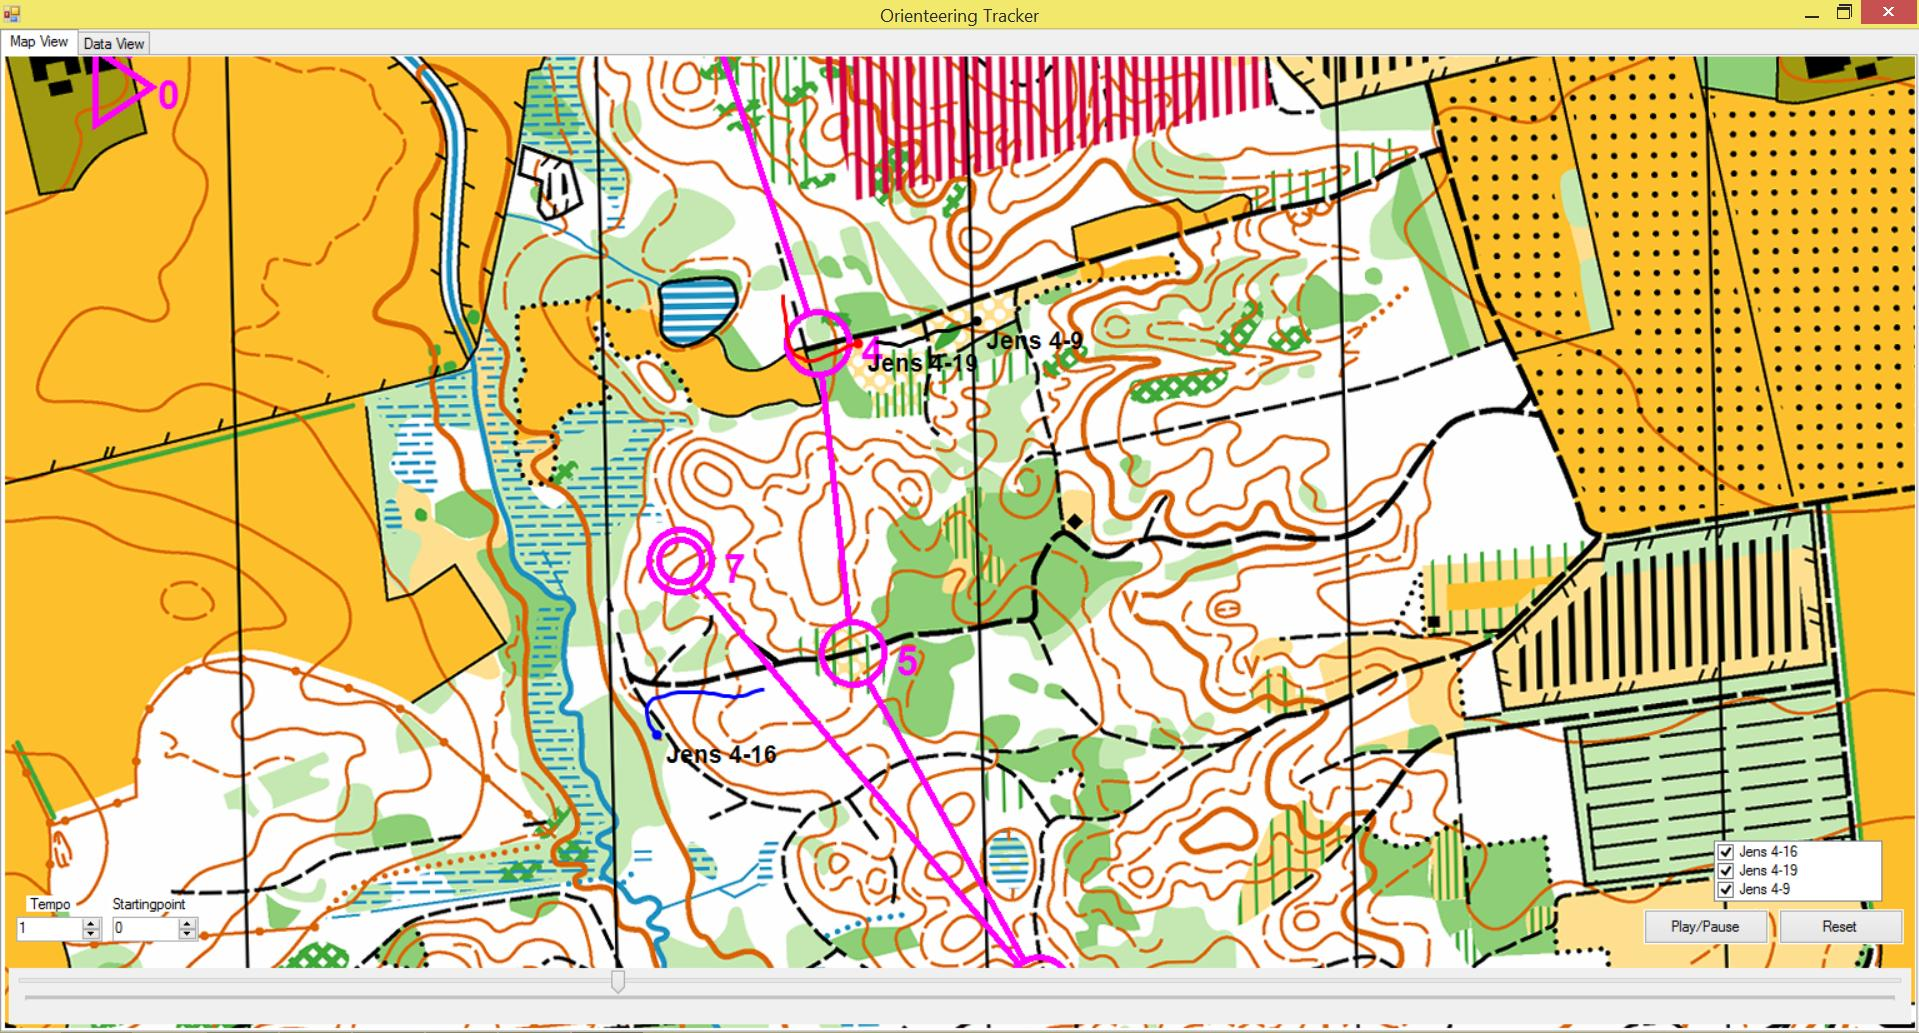
\includegraphics[width=1\textwidth]{billeder/MapView2}
	\caption{Klassediagram over projektets program}
\end{figure}

I bunden af programmet ses programmets trackbar, der gør det muligt at spole frem og tilbage under afspilningen. Nede i venstre hjørne findes to forskellige mediaplayer funktioner. Den yderste til venstre bruges til at vælge tempoet for afspilningen. Den anden bruges til at vælge startpost for løberne, hvilket gør det muligt at samle løberne, for lettere at kunne sammenligne dem med hinanden. På højre side ses en play/pause og  reset knap. Play/pause bruges til at starte/pause afspilningen. Reset knappen bringer programmet tilbage til dets opstarts stadie. Lige over disse to knapper findes en check box. I denne checkbox kan alle løberne ses. Checkboxen afgør hvilke løbere der vises på kortet, hvilket gør det muligt at skjule løbere, hvis der vil fokuseres på nogle bestemte løbere. Løberne vises ude på kortet med en prik i hver deres farve, samt en hale efter denne, som viser hvordan de har løbet de sidste 30 sekunder. 

Når der trykkes på tabben “Data View” vil alle løbernes data for løbet vises. I “Data View” kan der ses løbernes slut position, navn, tid, tidsdifference til førstepladsen, tilbagelagt distance, hastighed i minut pr. kilometer og tiden for hvert stræk. Der kan ses et eksempel på dette på figur 6.3 herunder. 
\begin{figure} [h]
	\centering
	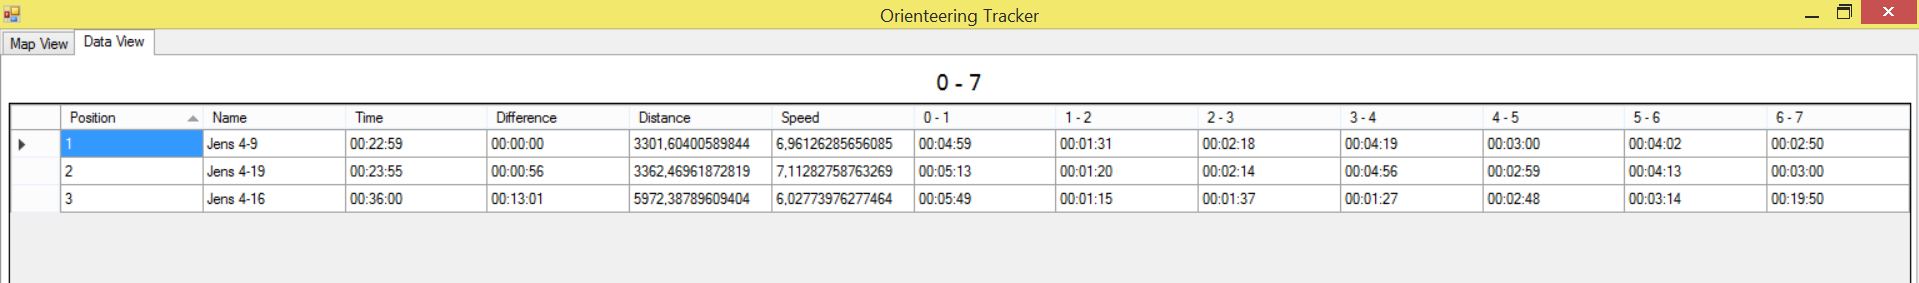
\includegraphics[width=1\textwidth]{billeder/DataView1}
	\caption{Klassediagram over projektets program}
\end{figure}

Klikkes der på et felt for et stræk, kan der ses mere detaljerede informationer om det specifikke stræk. Som det kan ses på figur 6.4, indeholder dette de samme informationer som når der ses på hele løbet, med en enkelt undtagelse, her kan løberne se hvilken position de fik på det specifikke stræk. 
\begin{figure} [h]
	\centering
	\includegraphics[width=1\textwidth]{billeder/DataView2}
	\caption{Klassediagram over projektets program}
\end{figure}

\section{Programstruktur}
Da ingen af medlemmerne i gruppen tidligere havde erfaring med udvikling af store applikationer i C\# og Windows Forms, blev meget af udviklingen lavet ud fra “trial and error” princippet. Med det menes at gruppen forsøgte sig meget frem, for at lære at bruge Windows Forms, og der ikke blev lavet en decideret plan eller design for programmet, før udviklingen blev påbegyndt. Dette medførte at store dele af programmet blev lavet i samme klasse, hvilket forårsagede et forholdsvist lavt abstraktionsniveau. 

\subsection{Klassebeskrivelse}
Gruppen har vha. Visual Studio udarbejdet et klassediagram, for at give et bedre overblik over programmets klasser. I firkanterne i klassediagrammet ses klassens navn, dens fields, properties og metoder.

\begin{figure} [h]
	\centering
	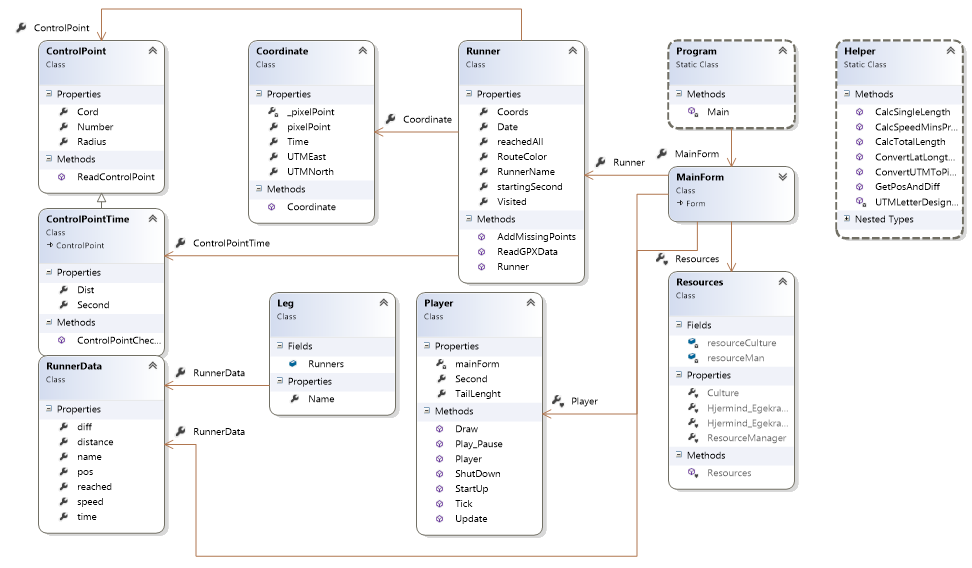
\includegraphics[width=1\textwidth]{billeder/KlasseDiagram}
	\caption{Klassediagram over projektets program}
\end{figure}

\begin {itemize}
\item \textbf{Helper} klassen indeholder de metoder der bruges til at lave udregninger i programmet, eksempelvis konverteringen fra  koordinater i længde- breddegrader til UTM koordinater. 
\item \textbf{Coordinate} indeholder koordinater for at kunne se hvor løberen er og hvor posterne er placeret, som både pixel- og UTM koordinater. 
\item \textbf{ControlPoint} repræsentere posterne i løbet. Den indeholder en posts radius, samt nummer og henter dens koordinater fra Coordinates.
\item \textbf{ControlPointTime} har nedarvet fra ControlPoint, den implementerer Second og Dist som vil være tid i sekunder og distancen fra løberen til posten. 
\item \textbf{Runner} indeholder informationer om en løber, dette er bl.a. løberens koordinater på ruten, om løberen har besøgt alle poster og løberens navn.
\item \textbf{RunnerData} gemmer på en mængde data om hver enkelt løber, som hastighed, distance løbet og position i løbet, dette vil være de informationer som kan findes under tabben som gruppen har kaldt ”Data view”. 
\item \textbf{Leg} er det engelske ord for ”stræk”.Leg indeholder en liste af RunnerData samt et navn på strækket.
\item \textbf{Player} sørger for at tegne løberen på kortet, samt den hale som skal være efter løberen. Derudover viser, skjuler og opdatere den forskellige funktioner i programmet når det køres. Dette bruges i den tab som gruppen har kaldt ”Map view”.
\item \textbf{MainForm} holder sammen på programmet. Det er her GUI’en bliver lavet og events bliver håndteret.
\item \textbf{Resources} indeholder kortet som bruges I programmet, samt world-filen.
\end {itemize}

Klasserne er kort beskrevet for at give et overblik over dem, og de vil blive beskrevet mere dybdegående i næste afsnit om ‘kildekoden’.

\section{Kildekoden}
I dette afsnit vil kildekoden til programmet blive beskrevet. Der vil være mere fokus på de større metoder i klasserne, frem for de mindre metoder.

\subsection{Helper}
Helper er en statisk klasse, der er lavet for at have nogle funktioner tilgængelige overalt i programmet, uden at skulle instantiere et nyt objekt der kunne udføre handlingerne, eller copy-paste funktionerne ind i de klasser der skal bruge dem. 

Helper indeholder konverteringsfunktionerne, i henholdsvis ConvertLatLongToUTM, og ConvertUTMToPixel. ConvertLatLongToUTM funktionen, er lånt fra brugeren Hactic fra Worldwindcentral's forum \citep{UTM}.
Derudover bliver Helper klassen også brugt til at lave beregninger på løbernes ture, altså distance og hastighedsberegninger.
 
ConvertUTMToPixel metoden konvertere UTM koordinatsæt, til en bestemt pixel på kortet. Metoden benytter formlerne beskrevet i teoriafsnittet, og en world-fil gemt i Resources.

\begin{lstlisting}
public static void ConvertUTMToPixel(double UTM_north, double UTM_east, out float x, out float y)
{
    MemoryStream ms = new MemoryStream(OrienteeringTracker.Properties.Resources.Hjermind_Egekrat_ref_ref1);
    string line;
    List<float> worldTal = new List<float>();
    StreamReader sr = new StreamReader(ms, Encoding.UTF8);

    while ((line = sr.ReadLine()) != null)
    {
        worldTal.Add(float.Parse(line, CultureInfo.InvariantCulture));
    }

    x = Convert.ToInt32((UTM_east - worldTal[4]) / worldTal[0]);
    y = Convert.ToInt32((UTM_north - worldTal[5]) / worldTal[3]);
}
\end{lstlisting}

\subsection{Coordinate}
Coordinate klassen indeholder både UTM koordinatsættet og pixel koordinatsættet. Derudover bliver en tid også gemt i Coordinate.

\subsection{ControlPoint}
Til at håndtere poster, er der lavet en klasse kaldet ControlPoint. Denne klasse indeholder et koordinat, Coord, for hvor posten befinder sig, og et nummer, Number, der indikere hvilket nummer i rækken, posten skal besøges. 
Derudover indeholder ControlPoint en funktion ReadControlPoint, der tager to parametre, line, en tekststreng der indeholder koordinaterne, og nr, denne posts nummer i rækkefølgen. 

\begin{lstlisting}
public void ReadControlPoint(string line, int nr)
{
    string[] coordinatesString = line.Split(';');
    this.Cord = new Coordinate(float.Parse(coordinatesString[2], System.Globalization.CultureInfo.InvariantCulture), float.Parse(coordinatesString[3], System.Globalization.CultureInfo.InvariantCulture), DateTime.Now, float.Parse(coordinatesString[0], System.Globalization.CultureInfo.InvariantCulture), float.Parse(coordinatesString[1], System.Globalization.CultureInfo.InvariantCulture));
    this.Number = nr;
}
\end{lstlisting}

\subsection{ControlPointTime}
ControlPointTime er en klasse der håndtere løbernes interaktion med posterne. ControlPointTime nedarver fra ControlPoint, og indeholder derfor de samme properties og metoder som ControlPoint. Derudover er der også tilføjet et sekund og en distance, der indikere hvornår løberen har nået den givne post, og hvor tæt vedkommende var på den. 

Metoden ControlPointChecker, tager et ControlPoint og en Runner, og tjekker om den pågældende løber rent faktisk rammer posten. Hvis den gør, så udfylder den data’en i instansen af ControlPointTime. 
Måden den gør det på, er ved at iterere igennem alle koordinaterne i løberens rute, indtil et af koordinaterne ligger inden for den givne radius af posten. Derefter tager funktionen alle de efterfølgende koordinater og ligger i en liste, indtil den igen rammer en der ikke er indenfor den givne radius af posten. 
Det koordinat der ligger tættest posten på fra den liste, bliver gemt som dataen i den nuværende ControlPointTime instans. 


\begin{lstlisting}
public void ControlPointChecker(ControlPoint cp, Runner r)
{
    List<ControlPointTime> distList = new List<ControlPointTime>();
    ControlPointTime cpt = new ControlPointTime();
    double doubleDist = 0;
    foreach (Coordinate coord in r.Coords)
    {
        doubleDist = Helper.CalcSingleLength(coord.pixelPoint.X, coord.pixelPoint.Y, cp.Cord.pixelPoint.X, cp.Cord.pixelPoint.Y);
        if (doubleDist < 25)
        {
            for (int i = r.Coords.IndexOf(coord); i < r.Coords.Count; i++)
            {
                if (Helper.CalcSingleLength(r.Coords[i].pixelPoint.X, r.Coords[i].pixelPoint.Y, cp.Cord.pixelPoint.X, cp.Cord.pixelPoint.Y) > 25)
                {
                    ControlPointTime thisCpt = distList.OrderBy(distance => distance.Dist).First();
                    this.Cord = thisCpt.Cord;
                    this.Dist = thisCpt.Dist;
                    this.Number = thisCpt.Number;
                    this.Second = thisCpt.Second;
                    this.Radius = thisCpt.Radius;
                    return;
                }
                cpt = new ControlPointTime();
                cpt.Cord = cp.Cord;
                cpt.Number = cp.Number;
                cpt.Second = r.Coords.IndexOf(coord);
                cpt.Dist = Helper.CalcSingleLength(r.Coords[i].pixelPoint.X, r.Coords[i].pixelPoint.Y, cp.Cord.pixelPoint.X, cp.Cord.pixelPoint.Y);
                cpt.Second = i;
                distList.Add(cpt);
            }    
        }
    }
    this.Cord = null;
    this.Dist = 0;
    this.Number = 0;
    this.Second = 0;
    this.Radius = 0;
    return;
}
\end{lstlisting}

\subsection{Runner}
Runner er en klasse til at repræsentere en løbers tur, der opbevare data om den rute løberen har løbet, tiden, distancen med videre. Den har følgende properties:

\begin{lstlisting}
public string RunnerName { get; set; }
public DateTime Date { get; set; }
public System.Drawing.Color RouteColor { get; set; }
public bool reachedAll { get; set; }
public List<int> startingSecond { get; set; }
public List<Coordinate> Coords { get; set; }
public List<ControlPointTime> Visited { get; set; }
\end{lstlisting}

Til at gemme ruten, er der på hver Runner lavet en liste af koordinater, kaldet Coords.
Disse koordinater er de punkter løberen har været på i løbet af sin tur, og bliver brugt både til at vise turen på et kort, og til at se hvor tæt løberen har været på posterne, for at se om vedkommende har nået disse punkter.
Derudover indeholder Runner klassen også en liste af ControlPointTimes. Denne liste hedder Visited, og indeholder data om hvorvidt løberen har nået en post. Hvis løberen har nået den pågældende post, ligger dataen i listen under det nummer som posten har. Hvis ikke, så indeholder ControlPointTime kun tomt data. 
 

Runner klassen indeholder også funktionalitet til at læse data fra en .gpx fil, altså en fil der indeholder data fra en gps-modtager, som fx en mobil der har været med på løbeturen.
Dette bliver gjort i følgende klassemetode, ReadGPXData:


\begin{lstlisting}
public void ReadGPXData(FileStream GpxStream)
{
	GpxReader reader = new GpxReader(GpxStream);
	reader.Read();
	this.Date = reader.Track.Segments[0].TrackPoints[0].Time;
	this.RunnerName = Path.GetFileNameWithoutExtension(GpxStream.Name);

	foreach (GpxPoint gp in reader.Track.Segments[0].TrackPoints)
	{
		double UTMNorthing;
		double UTMEasting;
		string Zone;
        Helper.ConvertLatLongtoUTM(gp.Latitude, gp.Longitude, out UTMNorthing, out UTMEasting, out Zone);

        float x;
        float y;
        Helper.ConvertUTMToPixel(UTMNorthing, UTMEasting, out x, out y);

        Coordinate c = new Coordinate(x, y, gp.Time, (float)(UTMEasting), (float)(UTMNorthing));
        this.Coords.Add(c);
        }
    GpxStream.Close();
    this.AddMissingPoints();
}
\end{lstlisting}

Denne metode bruger en GpxReader klasse, der stammer fra KILDE MANGLER. Readeren har en funktion der hedder Read, som ud fra en FileStream, altså en fil, læser de nødvendige data, og gemmer det i sin Track property. Denne Track property indeholder alle koordinaterne i en liste, men gemmer dem i længde- og breddegrader. Derfor bruges en hjælpefunktion fra en Helper-klassen, til at konvertere til UTM koordinater, og igen til pixels. Efter konverteringen gemmes koordinaterne i listen af koordinater, Coords, der blev beskrevet ovenfor. 
Efter koordinaterner er læst ind fra filen, kaldes metoden AddMissingPoints. Problemet med de GPX-filer der er blevet brugt i projektet, er at der ikke nødvendigvis er et koordinat for hvert sekund, men at der godt kan være sprunget et sekund eller flere over, hvis GPS-modtagelsen har været dårlig. AddMissingPoints udfylder de sekunder der ikke er noget data, så det fremstår som at løberen ikke bevæger sig. På den måde er det lettere at finde ud af hvor lang tid løberen har løbet, da starttidspunktet er kendt.
 
\subsection{RunnerData}
RunnerData indeholder en række informationer, som bruges i "Data View" tabben.

\subsection{Leg}
Leg klassen indeholder en liste af RunnerData, samt et navn på det specifikke Leg.

\subsection{Player}
Player klassen styrer den grafiske afspilningen af løbernes ruter. Player indeholder en reference til MainForm, så den kan bruge nogle af dens data. \newline
Player klassens vigtigste property er integeren “Second”. Denne property indeholder informationer om hvilket sekund programmet er kommet til i afspilningen, i forhold til startpunktet. 

Draw metoden sørger for at tegne de forskellige løberes position og hale ind på kortet.
Draw metoden iterere igennem alle Runner objekter i listen Runners fra MainForm, dvs. alle løbere.\newline
Først tjekkes at den pågældende Runner ikke er tjekket fra i checkboxen i Map View tabben, hvis dette er tilfældet hopper programmet videre til næste løber, og dermed vil denne løber ikke blive tegnet på kortet. \newline
Hvis løberen ikke er tjekket fra i checkboxen, tjekkes der efter om programmet er nået enden på gps data for løberen, hvis enden er nået, bliver denne løber ikke tegnet med på kortet.

\begin{lstlisting}
public void Draw(Graphics g)
{
    SolidBrush brush;
    Pen pen;
    int tempTailLenght = TailLenght;
    g.SmoothingMode = System.Drawing.Drawing2D.SmoothingMode.AntiAlias;

    foreach (Runner runner in mainForm.Runners)
    {
        if (!mainForm.RunnersCheckBox.CheckedItems.Contains(runner.RunnerName) || Second < 2
        || Second >= runner.Coords.Count() - runner.Visited[(int)mainForm.StartpointUpDown.Value].Second)
        {
                    continue;
        }

        brush = new SolidBrush(runner.RouteColor);
        pen = new Pen(brush, 3);

        if (Second < TailLenght)
        {
            tempTailLenght = Second;
        }

        PointF[] RunnerToDraw = new PointF[tempTailLenght];
        for (int Index = 0; Index < tempTailLenght; Index++)
        {
            RunnerToDraw[Index] = runner.Coords[Second - tempTailLenght + Index +
                runner.Visited[(int)mainForm.StartpointUpDown.Value].Second].pixelPoint;
            RunnerToDraw[Index].X *= mainForm.ZoomFactor;
            RunnerToDraw[Index].Y *= mainForm.ZoomFactor;
        }

        g.DrawLines(pen, RunnerToDraw);
        g.FillEllipse(brush, RunnerToDraw[RunnerToDraw.Length - 1].X - 4,
            RunnerToDraw[RunnerToDraw.Length - 1].Y - 4, 8, 8);
        g.DrawString(runner.RunnerName, new Font("Arial", 14, FontStyle.Bold), new SolidBrush(Color.Black),
            RunnerToDraw[RunnerToDraw.Length - 1].X + 5, RunnerToDraw[RunnerToDraw.Length - 1].Y + 5);
    }
}
\end{lstlisting}

Hvis programmet ikke er nået enden på data for løberen, laves der et nyt PointF array (PointF er et floating-point koordinatsæt), kaldet RunnerToDraw. Dette skyldes at metoden DrawLine fra Graphics klassen, tager et array af punkter ind og tegner en streg gennem alle disse punkter. Herefter indsættes de punkter der skal tegnes, på nuværende tidspunkt, ud fra Second propertien og startpunkt. Dette gøres i en for-løkke som iterere lige så mange gange som halen skal være lang, hvilket i dette program vil være 30. I for-løkken findes det ønskede punkt ved at indeksere Runner.Coords listen, udfra følgende formlen:
 
“Index i Coord listen” = “Sekunder fra startpunkt” - “halelængde” + “index fra for-lykken”  + “sekundet løberen passerede valgte startpunkt”

Grunden til at “sekundet løberen passerede valgte startpunkt” lægges til, skyldes at Second kun beskriver hvor lang tid der er gået siden valgte Startpunkt. 

Dernæst bliver RunnerToDraw’s X og Y koordinat multipliceret med ZoomFactor og bliver gemt som den nye X og Y værdi. Dette gøres så de indtegnede løbere følger med kortet, når der zoomes. 

Metoden Tick kaldes hver gang programmets timer ticker. Tick tjekker, om der er data fra Runners tilknyttet til det Second, programmet er nået til. Hvis ikke, stoppes timeren og TrackBarens indikator sættes lig det Second programmet er nået til, så den rykker sig med tiden kronologisk. Til sidst inkrementeres Second med 1.

\begin{lstlisting}
public void Tick()
{
    if (Second >= mainForm.Runners.Max(r => r.Coords.Count - r.Visited[(int)mainForm.StartpointUpDown.Value].Second))
    {
        mainForm.PlayTimer.Stop();
    }
    mainForm.PlayBar.Value = Second;
    mainForm.Map1.Refresh();
    Second++;
}
\end{lstlisting}

Derudover findes metoder som Play/Pause, Update, StartUp og ShutDown. Play/Pause bruges til at starte og stoppe afspilningen. Update opdatere hvor stor TrackBaren er, så den ikke kan trækkes længere end der er data til. StartUp viser alle mediaplayer funktionerne, hvor ShutDown skjuler alle mediaplayer funktionerne. 

\subsection{MainForm}
MainForm er hoved klassen i programmet og indeholder store dele af koden. Den håndtere UI’en og en del logik i programmet. 

Eventhandlerne Map1\_MouseMove og Map1\_MouseDown sørger for at kortet rykker sig, i takt med at brugeren trækker i kortet med venstre musetast holdt nede. 

Map1\_MouseWheel håndtere programmets zoomfunktion, ved at ændre på ZoomFactor, når brugeren scroller med musehjulet.

Map1\_MouseEnter sørger for at kortet har fokus, så snart musen er over kortet. 

LoadButton\_Click kaldes når “Load” knappen klikkes på, og viser en folder-browser-dialogbox til valg af mappe som indeholder GPX-data for løberne og GPS-data for ControlPoints. Efter valg af mappe, loades ControlPoints og GPX-data ind i systemet. Herefter skjules “Load” knappen, og mediaplayeren vises ved at kalde Player.StartUp().

PlayButton\_Click og PlayTimer\_Tick kalder henholdsvis Player.Play\_Pause() og Player.Tick().

Map1\_Paint sørger for, at kortets højde og bredde bliver skaleret efter ZoomFactor, så kortet tegnes i skaleret forhold, og kalder Player.Draw() og sender kortets grafik med.

PlayBar\_Scroll sørger for, at når brugeren trækker i TrackBar indikatoren følger Second med, på den måde er TrackBar og Second synkroniseret.

TempoUpDown\_ValueChanged ændre på intervallet mellem ticks for timeren, i forhold til værdien brugeren sætter det til. 

ResetButton\_Click sætter programmet tilbage til opstarts stadiet, når der trykkes på knappen, under kørslen af programmet. 

StartpointUpDown\_ValueChanged bestemmer startpunkt for afspilingen og sætter Second propertien til 0 og kører Player.Update som opdatere TrackBarens størrelse.

For at styre tabeloversigten over løbernes tid, position, hastighed osv., er der brugt en række funktioner. 
Den første hedder Setup\_Table, der ganske enkelt sætter overskrifterne i tabellen således:

DataTable.Columns[I].HeaderText = string;

De første 6 ændre sig aldrig, og bliver derfor hardcoded. Efter det, er resten af overskrifterne afhængige af om der bliver set på et delstræk, eller hele turen.  Til dette, er defineret en global variabel isLeg, der hele tiden holder styr på hvilket mode tabellen er i. Hvis det er et delstræk, bliver den sidste overskrift sat til ”Final position”, altså løberens endelige position i løbet. Hvis det derimod er hele løbet, sættes alle delstrækkenes navne til overskrifterne, fx ”1-2” eller ”2-3” osv. 

Derefter bruges funktionen Put\_Data, der tager et Leg som parameter. Det er vigtigt at bemærke at hele strækket fra start til slut, altså hele løbet, også er gemt som et Leg. Det er derfor variablen isLeg er nødvendig for at kunne skelne dem fra hinanden. Herefter bliver informationen for hver løber gemt i Leg, skrevet i tabellen. Der bliver tjekket om løberne har nået posterne, og tilføjet til tabellen på baggrund af den information. Derudover er der, som tidligere nævnt, forskel på om det kigges på et delstræk eller den samlede rute. I tilfældet hvor det er hele strækket der vises, bliver der i de første seks søjler, udskrevet den samlede information for løberne. I de resterende søjler, bliver udskrevet løbernes (rækker) tider i forhold til de pågældende delstræk  (søjler).

\begin{lstlisting}
private void Put_Data(Leg leg)
{
    DataTitle.Text = leg.Name;
    Setup_Table();
    DataTable.Rows.Clear();
    List<string> row;
    string time = "";
    string pos = "";
    foreach(RunnerData rd in leg.Runners)
    {
        if (rd.time <= new TimeSpan(0))
        {
            time = "X";
        }
        else
        {
            time = rd.time.ToString();
        }
        if (rd.pos == -1)
            pos = "X";
        else
            pos = rd.pos.ToString();
        if (isLeg)
        {
            row = new List<string> { pos, rd.name, time, rd.diff.ToString(), rd.distance.ToString(), rd.speed.ToString() };
            foreach (RunnerData mainRd in MainLeg.Runners)
            {
                if (mainRd.name == rd.name)
                {
                    if (mainRd.pos == -1)
                        row.Add("X");
                    else
                        row.Add(mainRd.pos.ToString());
                }
            } 
        }
        else
        {
            row = new List<string> { pos, rd.name, time, rd.diff.ToString(), rd.distance.ToString(), rd.speed.ToString() };
            foreach (Leg l in Legs)
            {
                for (int runnerIndex = 0; runnerIndex < l.Runners.Count; runnerIndex++)
                { 
                    if (rd.name == l.Runners[runnerIndex].name)
                    {
                        if (l.Runners[runnerIndex].time <= new TimeSpan(0))
                            time = "X";
                        else
                            time = l.Runners[runnerIndex].time.ToString();
                        row.Add(time);
                    }
                }
            }
                    
        }
        DataTable.Rows.Add(row.ToArray<string>());
    }
    DataTable.Sort(DataTable.Columns[0], ListSortDirection.Ascending);
}
\end{lstlisting}

LoadRunners  er en funktion der tager en række GPX filer ind som parametre, og opretter en Runner og RunnerData instans for hver fil. RunnerData der oprettes her, hører til i MainLeg, altså hele ruten og ikke bare et delstræk. 
Et foreach loop kører igennem hver fil i GPXFiles (inputparametren). En ny Runner oprettes, og ReadGPXData kaldes på instansen, for at fylde data i den pågældende Runner. Efter Runneren er oprettet,  kører endnu et foreach loop igennem alle ControlPoints, og opretter nye ControlPointTimes, ved at bruge funktionen ControlPointChecker. ControlPointTimes bliver tilføjet til Visited listen på Runner instansen.  En variabel, reached, holder styr på om løberen er nået igennem alle poster. 
En ny instans af RunnerData oprettes derefter, og hvis alle posterne er nået, altså reached siger sandt, udfyldes RunnerData med løberens data for sin tur. 
Efter dette er sket for alle GPX filer, kaldes GetPosAndDiff  metoden på Helper klassen, for at bestemme løbernes position, og differencen mellem dem. 

\begin{lstlisting}
private void LoadRunners(string[] GPXFiles)
{
    int ColorCount = 0;
    Runner runner;
    MainLeg.Name = string.Format("0 - {0}", ControlPoints.Count - 1);
    ControlPointTime cpt = new ControlPointTime();
    bool reached;

    foreach (string file in GPXFiles)
    {
        runner = new Runner();
        runner.ReadGPXData(new FileStream(file, FileMode.Open));
        runner.reachedAll = true;
        runner.RouteColor = Colors[ColorCount];
        ColorCount++;
        reached = true;


        foreach (ControlPoint cp in ControlPoints)
        {
            cpt = new ControlPointTime();
            cpt.ControlPointChecker(cp, runner);
            runner.Visited.Add(cpt);
            if (cpt.Cord == null)
            {
                reached = false;
            }
        }

        RunnerData runnerdata = new RunnerData();
        runnerdata.name = runner.RunnerName;
        if (reached)
        {
            runnerdata.distance = Helper.CalcTotalLength(runner, runner.Visited[0].Second,
                runner.Visited[runner.Visited.Count - 1].Second);
            runnerdata.time = TimeSpan.FromSeconds(runner.Visited[runner.Visited.Count - 1].Second -
                runner.Visited[0].Second);
            runnerdata.speed = Helper.CalcSpeedMinsPrKm(runnerdata.distance, (int)(runnerdata.time.TotalSeconds));
        }
        else
        {
            runnerdata.distance = 0;
            runnerdata.time = new TimeSpan(0);
            runnerdata.speed = 0;
        }

        runnerdata.reached = reached;
        MainLeg.Runners.Add(runnerdata);
        Runners.Add(runner);
    }
    MainLeg.Runners = Helper.GetPosAndDiff(MainLeg.Runners, Runners);
}
\end{lstlisting}

LoadControlPoints er en funktion der tager en fil som input, og bruger den til at oprette posterne i programmet. Ved et loop oprettes der en ny ControlPoint for hver linje i filen, og ReadControlPoint kaldes på det ControlPoint, og sender linjen fra tekstfilen med. 
Når posterne er læst ind, skal de tegnes på kortet. Et loop kører gennem ControlPoints listen, og der bliver tjekket for nummeret på posten. Hvis posten er den første tegnes en trekant, hvis posten er den sidste tegnes en cirkel inde i en cirkel, og ellers tegnes en enkelt cirkel. 
Et if-statement, tjekker til sidst om ControlPoint er den første i listen, og hvis ikke, så tegnes der en streg til den forrige. Dette gøres ved at beregne vinkel og distancen til den forrige post, og derefter tegne en streg baseret på den information. 

\begin{lstlisting}
private void LoadControlPoints(string RouteFile)
{
    ControlPoint newControlPoint;
    int cpNr = 0;
    foreach (var line in File.ReadLines(RouteFile))
    {
        newControlPoint = new ControlPoint();
        newControlPoint.ReadControlPoint(line, cpNr);
        ControlPoints.Add(newControlPoint);
        cpNr++;
    }

    Graphics g = Graphics.FromImage(Map1.Image);
    Pen p = new Pen(Color.Magenta);
    p.Width = 5;
    int i = 0;

    foreach (ControlPoint cp in ControlPoints)
    {
        Point[] points = {new Point(Convert.ToInt32(cp.Cord.pixelPoint.X + 30), Convert.ToInt32(cp.Cord.pixelPoint.Y)), 
                                    new Point(Convert.ToInt32(cp.Cord.pixelPoint.X - 15), Convert.ToInt32(cp.Cord.pixelPoint.Y-30)), 
                                    new Point(Convert.ToInt32(cp.Cord.pixelPoint.X - 15), Convert.ToInt32(cp.Cord.pixelPoint.Y+30))};
        if (ControlPoints.First() == cp)
        {
            g.DrawPolygon(p, points);
        }
        else if (ControlPoints.Last() == cp)
        {
            g.DrawEllipse(p, cp.Cord.pixelPoint.X - 17, cp.Cord.pixelPoint.Y - 17, 34, 34);
            g.DrawEllipse(p, cp.Cord.pixelPoint.X - 25, cp.Cord.pixelPoint.Y - 25, 50, 50);
        }
        else
        {
            g.DrawEllipse(p, cp.Cord.pixelPoint.X - 25, cp.Cord.pixelPoint.Y - 25, 50, 50);
        }


        using (Font myFont = new Font("Arial", 24, FontStyle.Bold))
        {
            g.DrawString(cp.Number.ToString(), myFont, Brushes.Magenta, new Point(Convert.ToInt32(cp.Cord.pixelPoint.X + 30),
                Convert.ToInt32(cp.Cord.pixelPoint.Y - 25 / 2)));
        }

        if (ControlPoints.First() != cp)
        {
            float xDiff = ControlPoints[i - 1].Cord.pixelPoint.X - cp.Cord.pixelPoint.X;
            float yDiff = ControlPoints[i - 1].Cord.pixelPoint.Y - cp.Cord.pixelPoint.Y;

            float angle = (float)Math.Atan2(yDiff, xDiff) - (float)(Math.PI);

            float distance = (float)Math.Sqrt(xDiff * xDiff + yDiff * yDiff);

            float newX = (float)(ControlPoints[i - 1].Cord.pixelPoint.X + (Math.Cos(angle) * (distance - 25)));
            float newY = (float)(ControlPoints[i - 1].Cord.pixelPoint.Y + (Math.Sin(angle) * (distance - 25)));

            g.DrawLine(p, new Point(Convert.ToInt32(ControlPoints[i - 1].Cord.pixelPoint.X + Math.Cos(angle) * 25),
                Convert.ToInt32(ControlPoints[i - 1].Cord.pixelPoint.Y + Math.Sin(angle) * 25)),
                new Point(Convert.ToInt32(newX), Convert.ToInt32(newY)));
        }
        i++;
    }
    Map1.Refresh();
}
\end{lstlisting}

LoadLegs indsætter data i listen Legs, der indeholder informationer om de enkelte stræk. Dette gøres ved at lave et for-loop for hvert ControlPoint, og inde i dette for-loop laves et foreach-loop for hver Runner i Runner listen. Inde i dette foreach-loop tjekkes, om den enkelte Runner har nået det specifikke ControlPoint. Hvis dette er opfyldt, bliver distance, tid og hastighed udregnet for det specifikke stræk og lægges ind i et nyt objekt af RunnerData klassen. Hvis dette ikke er opfyldt, bliver værdierne sat til 0. Herefter tilføjes RunnerData objektet til et Leg objekt, som indeholder information om alle Runners, for det enkelte stræk. Når alle Runners er blevet loadet ind, udregnes løbernes position i forhold til hinanden, og deres tids difference til den hurtigeste. Dette gøres vha. helper klassens GetPosAndDiff metode. Til sidst tilføjes dette stræk til listen Legs, som indeholder alle stræk. 

\begin{lstlisting}
private void LoadLegs()
{
    for (int i = 1; i < ControlPoints.Count; i++)
    {
        Leg leg = new Leg();
        leg.Name = string.Format("{0} - {1}", i - 1, i);
        foreach (Runner r in Runners)
        {
            RunnerData runnerdata = new RunnerData();
            if (r.Visited[i].Cord != null)
            {
                runnerdata.reached = true;
                runnerdata.distance = Helper.CalcTotalLength(r, r.Visited[i - 1].Second, r.Visited[i].Second);
                runnerdata.time = TimeSpan.FromSeconds(r.Visited[i].Second - r.Visited[i - 1].Second);
                runnerdata.speed = Helper.CalcSpeedMinsPrKm(runnerdata.distance, (int)(runnerdata.time.TotalSeconds));
            }
            else
            {
                runnerdata.reached = false;
                runnerdata.distance = 0;
                runnerdata.time = new TimeSpan(0);
                runnerdata.speed = 0;
            }

            runnerdata.name = r.RunnerName;
            leg.Runners.Add(runnerdata);
        }
        leg.Runners = Helper.GetPosAndDiff(leg.Runners, Runners);
        Legs.Add(leg);
    }
}
\end{lstlisting}







\chapter{Test}
\section{Monkey testning}
\begin{wrapfigure}{r}{0.5\textwidth}
	\begin{center}
		
\includegraphics[scale=0.75]{billeder/MonkeyTest}
	\end{center}
	\caption{Monkey testning}
\end{wrapfigure}
Denne test-type kan kategoriseres på forskellige måder, da der er forskellige typer af monkey testning. Der er Smart monkey test, og Ignorant monkey test (også kaldet Dumb monkey test), hvor begge typer er automatiske tests udført af software. De kategoriseres således:
Smart monkey test: Her gøres der brug af stokastisk unit test, da der laves test-suites, hvor ”aben” kender til input-type og ved hvilke metoder der skal testes. Denne test-type skal oftest købes, da det er mere avanceret software, som integreres med det kode som skal testes.
Smart monkey tests er hurtig til at finde fejl i programmet, hvis det er sat ordentligt op. Fejl fundet ved denne test-type er fra store til små, og kan typisk findes i en log-fil efter testen er kørt.
Ignorant monkey test: Denne test-type er en blackbox test, da den ikke har viden om programmets kode, og derfor tester random inputs på enhver mulig måde. Ignorant monkey tests kan findes som gratis software, bl.a. ”GUI tester”, som anvendes i dette projekt. ”Aben” kræver tæt på ingen opsætning af program for at kunne køre, og laver stress-test af programmet, og kan køre i flere dage, hvis ikke den finder fejl der får programmet til at crashe. Ved fejl i denne test, skal testeren typisk side og overvåge testen, da der typisk ikke er beskrivende log-filer over testen efter kørsel. Ignorant monkey test finder typisk store fejl i programmet, hvor de mindre fejl i koden ikke opdages. \citep{ExI}

\subsection{GUI tester}
GUI tester er et simpelt ignorant monkey test software, udviklet af Luigi Poderico, som er anvendt i dette projekt. Programmet køres ved at have det testede program i forgrunden, og derefter klikke på højre CTRL knap. GUI testeren vil herefter klikke på forskellige steder i programmet, og indtaste forskellige inputs hvis muligt. Problematikker ved dette software er, at det kan minimere test-programmet, åbne andre programmer, og prøve at ”teste” dem. \citep{GUItester} \newline
Ved brug af GUI tester i dette projekt, blev OrienteeringTracker startet, og GUI testen sat i gang. Der er lavet følgende tests:

1: Test uden at have manipuleret programmet. Der er her ikke loadet noget ind i programmet, og programmet består derfor kun af et kort, Map View tab, Data View tab og Load-knap. \newline
2: Test ved tryk af Load-knap, så dialogboksen åbnes, og testen derfor kan vælge hvilken som helst mappe.\newline
3: Test efter programmet har loadet filer. Her er både løbere, kort, poster og data tilstede i programmet.

I første testcase åbnes programmet, og GUI test startes. ”Aben” trykker mange steder, og ender med at minimere programmet flere gange før den får trykket på ”Load”-knappen. Der er ikke sket nogle fejl i programmet på dette stadie.\newline
I anden testcase har ”aben” klikket på Load, får valgt en mappe som ikke indeholder de rigtige filer, og programmet kaster en ArgumentNullException. Løsningen på denne fejl er at tjekke om filerne filtyperne er af .gpx og utm. \newline
I tredje testcase er de rigtige filer loadet ind i programmet, og ”aben” får lov til at teste både Map View og Data View. Den skifter selv mellem tabs, og prøver, i Map View, at indsætte forskellige værdier i både Tempo og Startpoint. Disse to værdier bliver derved sat til hhv. det mindst mulige (ved for lav værdi) eller det højest mulige (hvis værdien indsat er højere end muligt for programmet). Den slår nogle af løberne fra i checkboksen, og får både prøvet at starte løbet, og pauser løbet. I Data View valgte den en celle, og skrev en værdi i cellen. Dette skulle ikke ske, da en bruger da ville kunne manipulere med det viste. Dette blev ændret ved at gøre cellerne ReadOnly. ”Aben” får både klikket sig ind på et stræk, og gjort brug af tilbage-knappen.

\section{Blackbox testning}
Blackbox testning er en test-type, hvor testeren indtaster input til programmet, og ser på hvorvidt outputtet er korrekt. I dette projekt vil denne test-type bruges til at se, hvorvidt filer der loades ind håndteres korrekt. Her vil testcases indkludere følgende:

Testcase 1: Indlæsning af flere af samme person, for at observere hvorvidt Data View tabbet giver korrekt information, og hvordan flere personers rute afbildes i Map View. Her forventes, at Data View kan sorteres per kolonne, hvor en passende sortering finder sted, og at flere versioner af samme person kan afbildes i Map View uden exceptions.\newline
Testcase 2: Indlæsning af personer, som ikke når alle poster på ruten. Her forventes at deres data bliver sat til 0 eller ”X”.
Testcase 3: Lukke dialogboksen efter tryk på Load-knappen.


I testcase 1, hvor flere af samme person læses ind, bliver Map View vist korrekt, og alle ”personer” af samme persons rute, blev lagt ovenpå hinanden. I Data View blev data givet korrekt, men sortering af position gik galt. De øverste positioner ved sortering blev: 1, 10, 11, 12... 2, 21, 22... Dette skyldes, at sorteringen skete ved sammenligning af strenge, og ikke ved tal. (INDSÆT FIX HER).\newline
I testcase 2 blev personen, som ikke nåede alle poster, håndteret som forventet. Tider blev udskiftet med ”X” i de tilfælde personen ikke nåede en post, og difference i tid, samt distance løbet, blev sat til 0. Løberen indgår med korrekte tider i de stræk, som løberen nåede.
I testcase 3 crashede programmet med en ArgumentOutOfRangeException. Denne fejl blev rettet, ved at der ikke bliver loadet noget ind i programmet, før der bliver trykket "OK" i dialogboksen 




%% Afrunding %%

\chapter{Diskussion}





\chapter{Konklusion}
I gennem projektarbejdet med \textbf{\textit{IT i foreninger}}, har gruppen afgrænset til IT i o-løbsforeninger, og haft fokus på at optimere træningen for o-løbere. Gennem problemanalysen blev en række interessenter fundet, hvor der blev foretaget interview og mailkorrespondancer, for at finde frem til projektets problemstillinger. Projektets kravspecifikation blev udformet ud fra problemstillingerne, og blev afgrænset efter evner, erfaring og tid. Dette kapitel vil gennemgå om løsningsdelen overholder kravsspecifikationen og problemformuleringen.

Kravspecifikationen er opdelt i to dele. Den ene del er den grafiske afbildning, og den anden er en tekstbaseret afbildning.\newline
Programmets grafiske afbildning kan manipulere kortet, via zoom og flytning, afspille data, med pause og tempo funktioner, samt mulighed for at springe frem i afspilningen via en scrolling funktion (trackbar). Derudover findes funktionalitet til at til- og fravælge løbere, samt vælge hvilken post løberne skal samles og afspilles fra. Dette gør at programmet overholder alle krav for den grafiske afbildning. Dog er nogle kun delvist løst. Tempo-funktionaliteten er skaleret anderledes end beskrevet, ca. forhold: 1x, 4x, 9x, 16x, 25x. Brugeren har heller ikke mulighed for at tilpasse halelængden og farven på løberne. \newline
Programmets tekstbaserede afbildning viser de fleste af de ønskede informationer fra kravene. Kravet om visning af placering i løbet efter strækket og samlet tid efter strækket er ikke opfyldt. Der er blevet tilføjet information om placering for hele løbet til alle stræk.

Udover at kravspecifikationerne skal overholdes, skal projektets problemformuleringen også besvares, dette har kravspecifikationerne hjulpet med. Projektets problemformulering som er fundet frem til i problemanalysen, lød således:

Hvordan kan en telefonbaseret softwareløsning optimere evaluering og træning af o-løbere?
\begin{itemize}
	\item Hvordan kan løberne sammenlignes?
	\item Hvordan følges løberen rundt på ruten?
	\item Hvordan kan løsningen gøres brugervenlig?
\end{itemize}

OrienteeringTracker kan sammenligne løbere på to forskellige måder: Tekstbaseret, ved Data View, og grafisk ved Map View, som viser vejvalg m.m. \newline
Løberen kan følges på ruten gennem Map View, og som beskrevet i kravene, kan brugeren skifte mellem poster og hastighed. Dette gør, at brugeren kan sammenligne løbernes vejvalg på ruten synkront.
Efter afgrænsning fra krav til en optimal løsning, valgte gruppen at se bort fra brugervenlighed, til trods for at det er et vigtigt punkt i ethvert program.\newline
OrienteeringTracker er hidtil ikke et fuldt ud telefonbaseret softwareløsning, da programmet ikke er kørbart på en telefon. Dette skyldes, at gruppen har taget afstand fra applikationer til telefoner, og har derfor lavet et computer-program, og simuleret informationer der skulle sendes fra telefon-applikationen. Den simulerede information fra telefonen er givet ved en tredjeparts applikation.\newline
Programmet optimerer evaluering og træning af o-løbere, da det giver mulighed for sammenligning af både vejvalg, tider, hastighed og mere.
%%%% Kilder %%%%

\begingroup
	\raggedright
	\bibliography{bibtex/litteratur}							% Litteraturlisten inkluderes
\endgroup


%%%% Fixme-listen %%%%

%\newpage														% Ny side til Fixme-listen
%\listoffixmes													% Fixme-listen - fjernes til sidst i projektet med "%"


%%%% Appendiks %%%%

\appendix														% Appendiks/bilag start - giver chapter bogstaver i stedet for tal
\clearforchapter												% Sikrer at pagestylen aktiveres paa den rigtige side
\phantomsection													% Kunstigt afsnit, som hyperlinks kan 'holde fast i'
\pdfbookmark[0]{Appendiks}{appendiks}							% Tildeler en klikbar bookmark til den endelige PDF

%% Indstillinger for appendiks (deaktiveret med "%") %%

%\pagestyle{empty}												% Sidehoved/-fod for standardsider aendres til tom for appendiks
%\aliaspagestyle{chapter}{empty}								% Sidehoved/-fod for kapitelsider aendres til tom for appendiks
%\settocdepth{chapter}											% Kun kapitel-niveau vises i ToC
%\addtocontents{toc}{\protect\cftpagenumbersoff{chapter}}		% Sidetal for kapitler fjernes i ToC

%% Filer til appendiks %%

%%%% Bilag %%%%
%\phantomsection												% Kunstigt afsnit, som hyperlinks kan 'holde fast i'
%\addcontentsline{toc}{Bilag}{bliag} 				% Manuelle indgange i indholdsfortegnelsen (naar \includepdf bruges)

%\includepdf[pages={x-y}]{filnavn}								% Inkluder eksterne bilag med \includepdf[pages={x-y}]{filnavn}
%\chapter{Interviewguide}

\chapter{Interview transskribering}
Dette er et interview med Claus Bobach, foretaget af Frederik, Mark og Søren. 

Søren: Vi går på software på Aalborg Universitet, og har valgt et projekt som skal omhandle små foreninger, og Jens Børsting foreslog at tage kontakt til dig.\newline
Frederik: Lige nu er vi i en fase, hvor vi forestiller os en form for hjælp med jeres træning, med noget udstyr og software. Så vi vil gerne have dig til at fortælle lidt om hvordan en træningsgang forløber. Så kunne vi senere snakke om du har nogle forestillinger om, hvad der kunne hjælpe til træning, af software. Så hvis du kan forklare os hvordan en træningsgang forløber, helt fra i planlægger den, til udførelse og efter udførelsen.\newline
Claus: Vi starter med et blankt kort, på et program der hedder Ocad, der har vi så et program til at lægge lagene ovenpå, Condes, et forholdsvis simpelt program som er udvidet så mange gange at det er blevet rigtig godt. Her har vi mulighed for at lægge en simpel bane, eller noget mere kompliceret som at fjerne dele af kortet. Disse to programmer har så inden for de seneste år kunnet arbejde sammen, og de lag der så ligger i Ocad er delt om i farver og symboler, og i Condes kan man så bestemme hvad af det man vil have med. Så kan man eventuelt vælge kun at se kurvebilledet, når de to programmer arbejder sammen. Hvis ikke man har en cad-fil, så kan man bruge JPG filer, men så har man ikke samme mulighed for at ændre kortet. 
Så når jeg har lavet banen på et kort, så sender jeg det videre til en som printer det, og sender det til dem som sætter posterne ud. Jeg har så en stak kort til de folk som møder op. Så løber folk ellers ind i skoven og kommer hjem igen. \newline
Til de fleste træninger står folk selv for at skulle tage tid, hvis det er noget de vil. På de ugentlige træninger har vi ikke noget tidstagnings udstyr. Det har vi dog til de lidt mere specielle træninger, blandt andet traditionsløb og sådan, hvor vi har elektroniske enheder ude ved posterne. Her har vi så en enhed vi kan se det hele på, og printe ud fra. \newline
Frederik: Kan du sige lidt om, hvor lang tid det tager at lave kort og sætte poster ud?\newline
Claus: Jeg bruger normalt en time eller halvanden på at lave de tre baner vi løber på til almindelig træning, men vi har en gruppe på otte som skiftes til at sætte posterne ud. At sætte posterne ud tager typisk et sted mellem halvanden til to timer. Så der er selvfølgeligt noget forberedelse. Også i form af at hente posterne igen, men det prøver vi på at gøre i forbindelse med træningen. For eksempel i dag, der løb jeg bare som den bagerste og samlede posterne ind.\newline
Frederik: Du sagde, at i kunne vælge kun at have højdekurverne på kortet. Hvordan er dette relevant?\newline
Claus: Blandt andet her om onsdagen, der prøver vi på at øve forskellige teknikker, nu hvor orienteringsløb er rimelig komplekst, så vi deler det lidt op, så man kan øve forskellige ting. Det er der vi bruger det. Kurvebilledet er en af de ting der er vigtige at træne og læse. Så for at få det mere simpelt til træningen, har vi nogle gange kun kurvebilledet på kortet.\newline
Søren: Når i skal evaluere hvordan i løber, hvordan gør i det?\newline
Claus: Det optimale er selvfølgeligt at vi havde enheder på hver enkelte post hver gang, men det tager allerede halvanden time til to timer at sætte poster ud, og hvis vi så skal have enheder med hver gang, tager det en hel time mere. Og det at løbe bagerst og samle posterne ind, vil heller ikke være lige så nemt. Men der er to muligheder, som man også kan kombinere, men at bruge tiderne mellem de enkelte poster eller at bruge GPS-ur er de to muligheder der typisk bruges. Så de fleste scanner bare kortet ind og lægger GPS-dataen oven i.\newline
Frederik:  Ved du hvilket program de bruger til det? Altså til at samle GPS dataen.\newline
Claus: Der er en orienteringsløber oppe i Stokholm, eller sådan noget, det hedder Quickroute. Hvor han henter alt data hjem der ligger i gps uret, det vil sige puls og højde osv. Så man kan få graferne sammen og få det visuelt på kortet at hvis man eksempelvis vælger hastighed, så har løberen en skala fra rød til grøn.\newline
Frederik: Så man kan se hvor man har løber hurtigt og langsomt?\newline
Claus: Ja. \newline
Frederik: Okay. Kan den replay det? Altså så man kan se hvor langt man kom?\newline
Claus: Ja, jeg har faktisk ikke prøvet funktionen, men ja. Jeg tror han har lavet det og lavet det i forbindelse med Google Earth. Hvor Quickroute ligger o-kortet ind i Google Earth også laver den en replay der. \newline
Frederik: Okay, det tror jeg vi skal have kigget nærmere på hvad det er for noget. \newline
Claus: Der er helt klart også noget interessant der.\newline
Frederik: Når i nu ikke har tidtagning med der ude, hvordan evaluere i så bagefter? Det er måske bare lidt for at få erfaringen og holde formen ved lige?\newline
Claus: En ting er jo at nogle har deres GPS ur og selv går hjem og evaluere, men vi opfordre selvfølgelig også folk til at snakke sammen. Bare det at have set hinanden i skoven, kan man godt fornemme hvilke udfordringer de andre har haft. Det man har gjort helt tilbage fra starten af, er jo man har sat sig ned og snakket om hvad gjorde du og hvad gjorde jeg. \newline
Søren: Så vidt som de kan huske selvfølgelig.\newline
Claus: Ja selvfølgelig. \newline
Søren: Hvad med andre redskaber der kan bruge til at evaluere folk i deres træning?\newline
Frederik: Er der f.eks. nogle der bruger deres mobil telefon?\newline
Claus: Jeg tror det er mest til GPS urene, der er nok nogle få der bruger Endomondo, men ellers tror jeg ikke det er noget der er så udbredt. Det er så det Quickroute, hvor det er meget for den individuelle løber. Der er også nogle andre programmer, hvor arrangørerne, altså efter en konkurrence, at de lægger et kort op, hvor alle så kan lægge deres GPS rute ind oven i. De bliver desværre ikke brugt så voldsomt meget lige i forløbet, det var meget populært for en 3-4-5 år siden. Det var som om der var et enkelt program som var rigtig brugervenligt, som folk brugte, men det var der så åbenbart ikke økonomi i, så det svenske forbund valgte at begynde at bruge noget andet, det har man så ikke rigtig for arrangører og løber ind til at støtte op om. Det kræver så, for virkelig at få noget ud af det, skal man have 20-30\% af løberne til at bruge det. \newline
Frederik: Ja okay, det er vigtigt de alle sammen er med på det. 
Claus: Ja, så derfor kan det godt være vigtigt som arrangør, hvor vi nu skal arrangere et løb her om 2½ uge for 1.500 løbere, hvis vi f.eks. som vi nogle gange har gjort lægger kortet op i et af de der programmer, så er det vigtigt at vi reklamere for det, ellers bliver det jo bare udvasket. \newline
Frederik: Kan du huske hvad det hed?\newline
Claus: Altså det de stoppede med at bruge, det hed RunOWay.\newline
Søren: Vi har også hørt om TracTrac, om det er noget der er udbredt? Men som vi kunne forstå, var det forholdsvist dyrt. \newline
Claus: Det bliver mest brugt til at live rapportere. Enten hvis vi sidder der hjemme, når der er VM et eller andet sted ude i verden, så kan vi se med hvor. De bruger det også til at have en stormskærm på pladsen, når der er konkurrencer. \newline
Frederik: Det er mest til større events?\newline
Claus: Ja det er det. Jeg er lidt i tvivl om landsholdet måske, har brugt det lidt.\newline
Frederik: Jeg tror de bruger det, det mente Jens Børsting i hvert fald.\newline
Claus: Det tror jeg faktisk også. Det udstyr der bliver brugt til de store konkurrencer herhjemme, har landsholdet jo til dagligt. Så jeg tror måske de bruger det lidt, men jeg ved faktisk ikke hvor meget.\newline 
Frederik: Jeg tænkte om du måske havde nogle idéer til områder, hvor du kunne forestille dig der var et eller andet en eller anden form for optimering i forhold til noget software du havde tænkt over? Inden vi snakker vores idé. \newline
Claus: Vi har et enkelt problem i øjeblikket, men det tror jeg også er lidt et spørgsmål om vilje herfra. Når vi arrangere et o-løb herfra, så for at få data ind fra skoven, ikke GPS data, men bare tidsdata, bare fra en enkelt post eller to, så er vi meget afhængige af… Det er vi nød til at kable ud til. Altså, at vi decideret har et fysisk kabel, og det begrænser lidt muligheden for hvor langt udefra man kan få meldingen. Så der vil vi jo gerne have en enhed som kunne sende det, eller nogle programmer der kan håndtere det, for jeg tror nok at enheden findes. Jeg tror nok de bruger det nede i Sønderjylland, men de bruger et andet program der skal modtage det. Så det, ja, det er en af vores udfordringer i øjeblikket. \newline
Mark: Men er det i forbindelse med at få data direkte, eller når i kommer tilbage og skal evaluere.\newline
Claus: Det er med det samme. Vi har en mand på pladsen der sidder og speaker om hvordan det går. Lige nu bruger vi det bare sådan at han har en forvarsling på hvem der kommer næst, altså så han kan forberede sig, men specielt på de lange distancer ville det være rart at have en post halvvejs han kunne speake nogle tider fra.\newline
Frederik: Ja men vi kunne måske snakke lidt om hvad vi har tænkt på. 
En af de første ting vi tænker, var virtuelle poster, hvor du får en form for lyd, når du er i nærheden. Men vi fandt noget der faktisk var det vi havde forestillet os, og hvis det er ude, og det ikke bliver brugt, så tænkte vi at det nok ikke var noget der var så aktuelt.I stedet, så vil vi gerne prøve at lave noget der ligne TracTrac, hvor du bruger din mobil som GPS-sender, for så vidst vi har forstået, så er der ikke nogle af GPS-urene der kan sende data direkte. Nu må vi se hvor præcise GPS’erne i mobilerne er, men så ville det jo være noget man kunne gøre live, og så ville det være noget hvor man, igen som du siger, lave en eller anden form for program som arrangørerne laver, og så få lagt kort ind, og få samlet alle folk ruter og sådan nogle ting, så de kan sammenligne, meget ligesom TracTrac, men så prøve at gøre det lidt billigere fordi det er via mobilen. Men det ved jeg ikke hvad du tænker om?\newline
Claus: Jamen det tror jeg da helt klart kunne være interessant.\newline
Frederik: Er det noget til sådan en almindelig træning som i dag, tror du der er nogle der ville bruge det der, eller ville det være til arrangerementer?\newline
Claus: Altså det live mæssige ville vi nok ikke bruge til træning, men jo hvis det er noget man nemt bagefter ville kunne tage frem, så tror jeg da helt sikkert at det… \newline
Frederik: Altså jeg tænkte at hvis man nu havde en projekter op her på væggen, så kunne man…\newline
Claus:  Så kunne man bruge det umildbart efter ja.\newline
Frederik: Det var i hvert fald det vi havde i tankerne\newline
Claus: Jamen det er da rigtigt, det tror jeg godt man kunne få nogle til at bruge\newline
Frederik: Så er i også fri for de der tidtagninger ude i skoven, så behøver i ikke dem. Så kan i jo bare se.\newline
Claus: Nej nej\newline
Frederik: Det er vores tanke lige nu\newline
Claus: Der er nogle af de der, der har gjort noget lignende. Det vi bruger posterne ude i skoven til, er jo at få mellemtider. Der er nogle af de der programmer der faktisk har kunne gøre det ved hjælp af GPS’en. \newline
Frederik: Så den registrere om man er kommet tæt nok på posten, og at man så regner med at man har fundet den.\newline
Claus: Ja, et eller andet estimat af hvornår folk har været ved posten, så man ved hvor lang tid man har brugt mellem posterne, uden at man skal sidde og.. ja..\newline
Søren: Jeg tror egentlig også vores primære ide, var at man kunne sammenligne de vejvalg og de stræk man tager, så vi kunne tage fra en post, og…\newline
Claus:  Ja ja\newline
Frederik:  Jeg havde ikke tænkt over den med at det tager længere tid for jer at sætte de poster ud der skal brik til, end dem der ikke skal, men det er klart. \newline
Claus: Men det gør det. Fordi det vi sætter ud nu, det er skærme i den her størrelse, det koster jo ingenting at have med. \newline
Frederik:  Så du skal selv ligesom, hvad skal man sige. Der er ikke noget papir for at validere at du har været derude. \newline
Claus: Nej, vi hænger heller ikke stifteklemmer derude, for det er jo også. Hvis du løber rundt med nogle poster med en snor på, og der hænger noget tungt ude for enden, så i løbet af 5 minutter, så er de snore viklet sammen.\newline
Frederik: Jeg tror heller ikke vi har så meget mere.\newline
Søren: Nej, egentlig ikke.\newline
Frederik: Så er det pizza tid!\newline 

\chapter{E-mail korrespondance med Jens Børsting}
\textbf{Hvordan foregår en træningsgang af o-løb?}\newline
Man starter med at få en skovtilladelse hvor løbet skal foregå.
Træneren beslutter hvad der skal trænes og planlægger løbet i et computer program der hedder ”Condes”. Her lægges baner og tegnes kort. Herefter udskrives kort for alle de baner der skal løbes. Dette inkluderer et kort til udsætning af alle poster. Det meste af dette arbejde kan gøres hjemmefra. Dog er det ofte sekretæren i klubben der printer kortene.
Typisk dagen før træningen hentes alle poster i klubhuset og sættes ud i skoven.
På træningsdagen mødes alle løbere og får instruktion i løbets momenter i dag og baner fordeles alt efter niveau og kondition. Typisk vil der være 3-7 baner at vælge imellem.
Løberne sendes i skoven. Alle løber med en elektronisk brik der registrere hvornår man har været ved her post.
Ved hjemkomst får man en udskrift over hvilke poster man har været ved og hvor lang tid der er gået mellem hver post (stræktider)
Man har så mulighed for at gennemgå løbet ved at snakke med andre løbere og trænerne. Her diskuteres vejvalg og hvad der gik godt og hvad der gik mindre godt. Stræktider sammenlignes. Vejvalg foregår udelukkende efter hukommelse og det er ikke muligt at se forskel i hastighed på kortere stræk end hele strækket mellem 2 poster.
Hvis løberen ikke er sikker på hvor han/hun har været kan det være meget svært at analysere hvad der gik galt.
Dagen efter løbet skal alt udstyret der er placeret i skoven hentes ind igen og pakkes ned i klubhuset hvis det ikke skal hænges til tørre først.

\textbf{Hvordan evaluerer trænere deres løbere? (Hvad vurderer han på, og hvordan observerer han dette?)}\newline
Eneste mulighed træneren har er at snakke med løberen efter løbet og ud fra stræktider og løberens hukommelse af vejvalg diskutere hvad der virkede og hvad der ikke gjorde.

\textbf{Hvordan evaluere respondenten sin egen tur? (hvordan kan respondenten selv se fremskridt eller fejl ved sin egen træning?)}\newline
På samme måde som med træneren kan løberen læse sine stræktider og evt. sammenligne med andre løbere der har løbet sammen stræk. Det kræver dog at disse løbere er til stede. Ved de ugentlige træninger bliver stræktider ikke offentliggjort, så man kan ikke sammenligne online efter løbet. Ved større løb bliver alle stræktider offentliggjort på nettet og man kan sidde hjemme i ro og mag senere og analysere sit løb i forhold til andre. Det er vigtigt at man kan sammenligne med andre da der er stor forskel på løbsterræn og dermed hastighed i terræn ved forskellige løb. Man kan dog sammenligne med dem man normalt lige op med løber med og kan se om man har løbet hurtigere eller langsommere end den på dette løb i forhold til tidligere løb.

\textbf{Hvordan kan denne evaluering gøres mere præcis, eller endda indkludere flere aspekter af løbet?} \newline
Ved at have gps tracking som kan følges live under løbet kan træneren se hvordan løbet forløber og nemmere snakke vejvalg og andet teknisk træning efter løbet. Evt. kan vejledning gives under løbet, hvis løberen er faret helt vild. Tracks kan sammenlignes med andre for at se hvor på strækket der har været fart på og hvor der ikke har. Samlet afspilning af løberne fra en post til en anden kan give et godt billede af udviklingen af løbet.
Det at have gps med på løbet kan også give mulighed for at give elektronisk tilbagemelding om at man er ved posten, kan man reducere arbejdsmængden ved udsætning og indhentning af poster. Samtidig er løberen uafhængig af hvornår der er poster i skoven og kan løbe løbet når det passer ham (dog skal der være løbstilladelse i skoven).

\textbf{Hvilke redskaber og metoder kender respondenten til, og hvilke bliver generelt set brugt i træningen?}\newline
Kort, stræktider og hukommelse er det normale. Sammenligning af stræktider med andre ved løbets afslutning eller ved større løb online hjemme i de efterfølgende dage.
Nogle få kender til Travel Tales og PDFmaps, men det bliver stort set aldrig brugt da det ikke giver en samlet løsning.
TracTrac og lignende systemer bliver kun brugt at landsholdsløbere og til nogle få eliteløbere til de store stævner.

\textbf{Hvordan mener respondenten, at en træningsgang kan blive optimeret? (Hvilke evaluerings punkter er mangelfulde)}\newline
Ved at kunne sammenligne gps tracks kan man nemmere vurdere om hvilke vejvalg der har virket og hvor det er gået galt/langsomt. Her kan man se om det kunne betale sig at løbe udenom eller det var nemmere at løbe igennem en tæthed eller over en stejl bakke mv.
\chapter{Nyt P2 forslag}


\end{document}													% Slutter dokumentet - obligatorisk


